% !Mode:: "TeX:UTF-8"
%% 请使用 XeLaTeX 编译本文.
% \documentclass{WHUBachelor}% 选项 forprint: 交付打印时添加, 避免彩色链接字迹打印偏淡. 即使用下一行:
\documentclass[forprint]{WHUBachelor}
\usepackage{geometry}
\usepackage{float}
\usepackage{minted}

\begin{document}
%%%%%%% 下面的内容, 据实填空.

\title{基于Digilent Nexys 4 DDR的CPU设计\\ {\Large《计算机设计与实践》实验五报告}}
\author{马玉坤}                            % 作者名字
\Cmajor{计算机科学与技术}                  % 专业中文名
\Cschoolname{计算机科学与技术系}          % 学院名
\date{二〇一七年七月}                    % 日期, 要注意和英文日期一致!!

%-----------------------------------------------------------------------------
\pdfbookmark[0]{封面}{title}         % 封面页加到 pdf 书签
\frontmatter
\pagenumbering{Roman}              % 正文之前的页码用大写罗马字母编号.
%-----------------------------------------------------------------------------
% !Mode:: "TeX:UTF-8"

%%% 此部分需要自行填写: (1) 中文摘要及关键词 (2) 英文摘要及关键词

%%======中文摘要===========================%
\begin{cnabstract}
  在本次CPU设计过程中,本人在两位实验课老师和Digilent社区的帮助下,设计了一个可在Nexys 4 DDR上运行的,有固定指令周期的且支持十条指令的精简指令集 (RISC) 处理器。本文详细介绍了本人在计算机设计与实践实验课上完成计算机设计与实践实验5的相关设计。本文内容包括: (1) CPU的顶层设计; (2) CPU各个模块,包括取指模块、运算模块、访存模块、回写模块、内存控制以及IO控制若干个模块的内部设计; (3)进行CPU设计及实现过程中遇到的问题与解决方法; (4) Digilent Nexys 4 DDR FPGA的简单介绍。

\end{cnabstract}
\par
\vspace*{2em}


%%%%--  关键词 -----------------------------------------%%%%%%%%
%%%%-- 注意: 每个关键词之间用“;”分开,最后一个关键词不打标点符号
\cnkeywords{中央处理器; CPU; FPGA; VHDL; 计算机设计与实践 }
    % 加入摘要, 申明.
%==========================把目录加入到书签==============================%%%%%%
\pdfbookmark[0]{目录}{toc}
\tableofcontents
\mainmatter %% 以下是正文
%%%%%%%%%%%%%%%%%%%%%%%%%%%--------main matter-------%%%%%%%%%%%%%%%%%%%%%%%%%%%%%%%%%%%%

\chapter{CPU的顶端结构}

如图\ref{fig:cpu_top}所示,整个CPU由时钟管理、取指管理、运算管理、访存管理、回写管理、访存控制以及IO控制七个模块组成。每个模块相对独立(有独立的输入和输出)又同时紧密联系(输入输出端口相连)。

在图\ref{fig:cpu_top}中,信号线的约定如下:
\begin{enumerate}[1)]
\item 所有信号线中,宽度为1位的,例如CLK、RST信号,都用细线表示。
\item 所有信号线中,宽度为8位的,例如RTEMP、ALU\_out,都用较粗的线表示。
\item 所有信号线中,宽度为16位的,例如ADDR、IR、PC,都用最粗的线表示。
\end{enumerate}

\newgeometry{left=0.3cm, right=0.3cm, top=0.3cm}
\begin{figure}
  \centering
  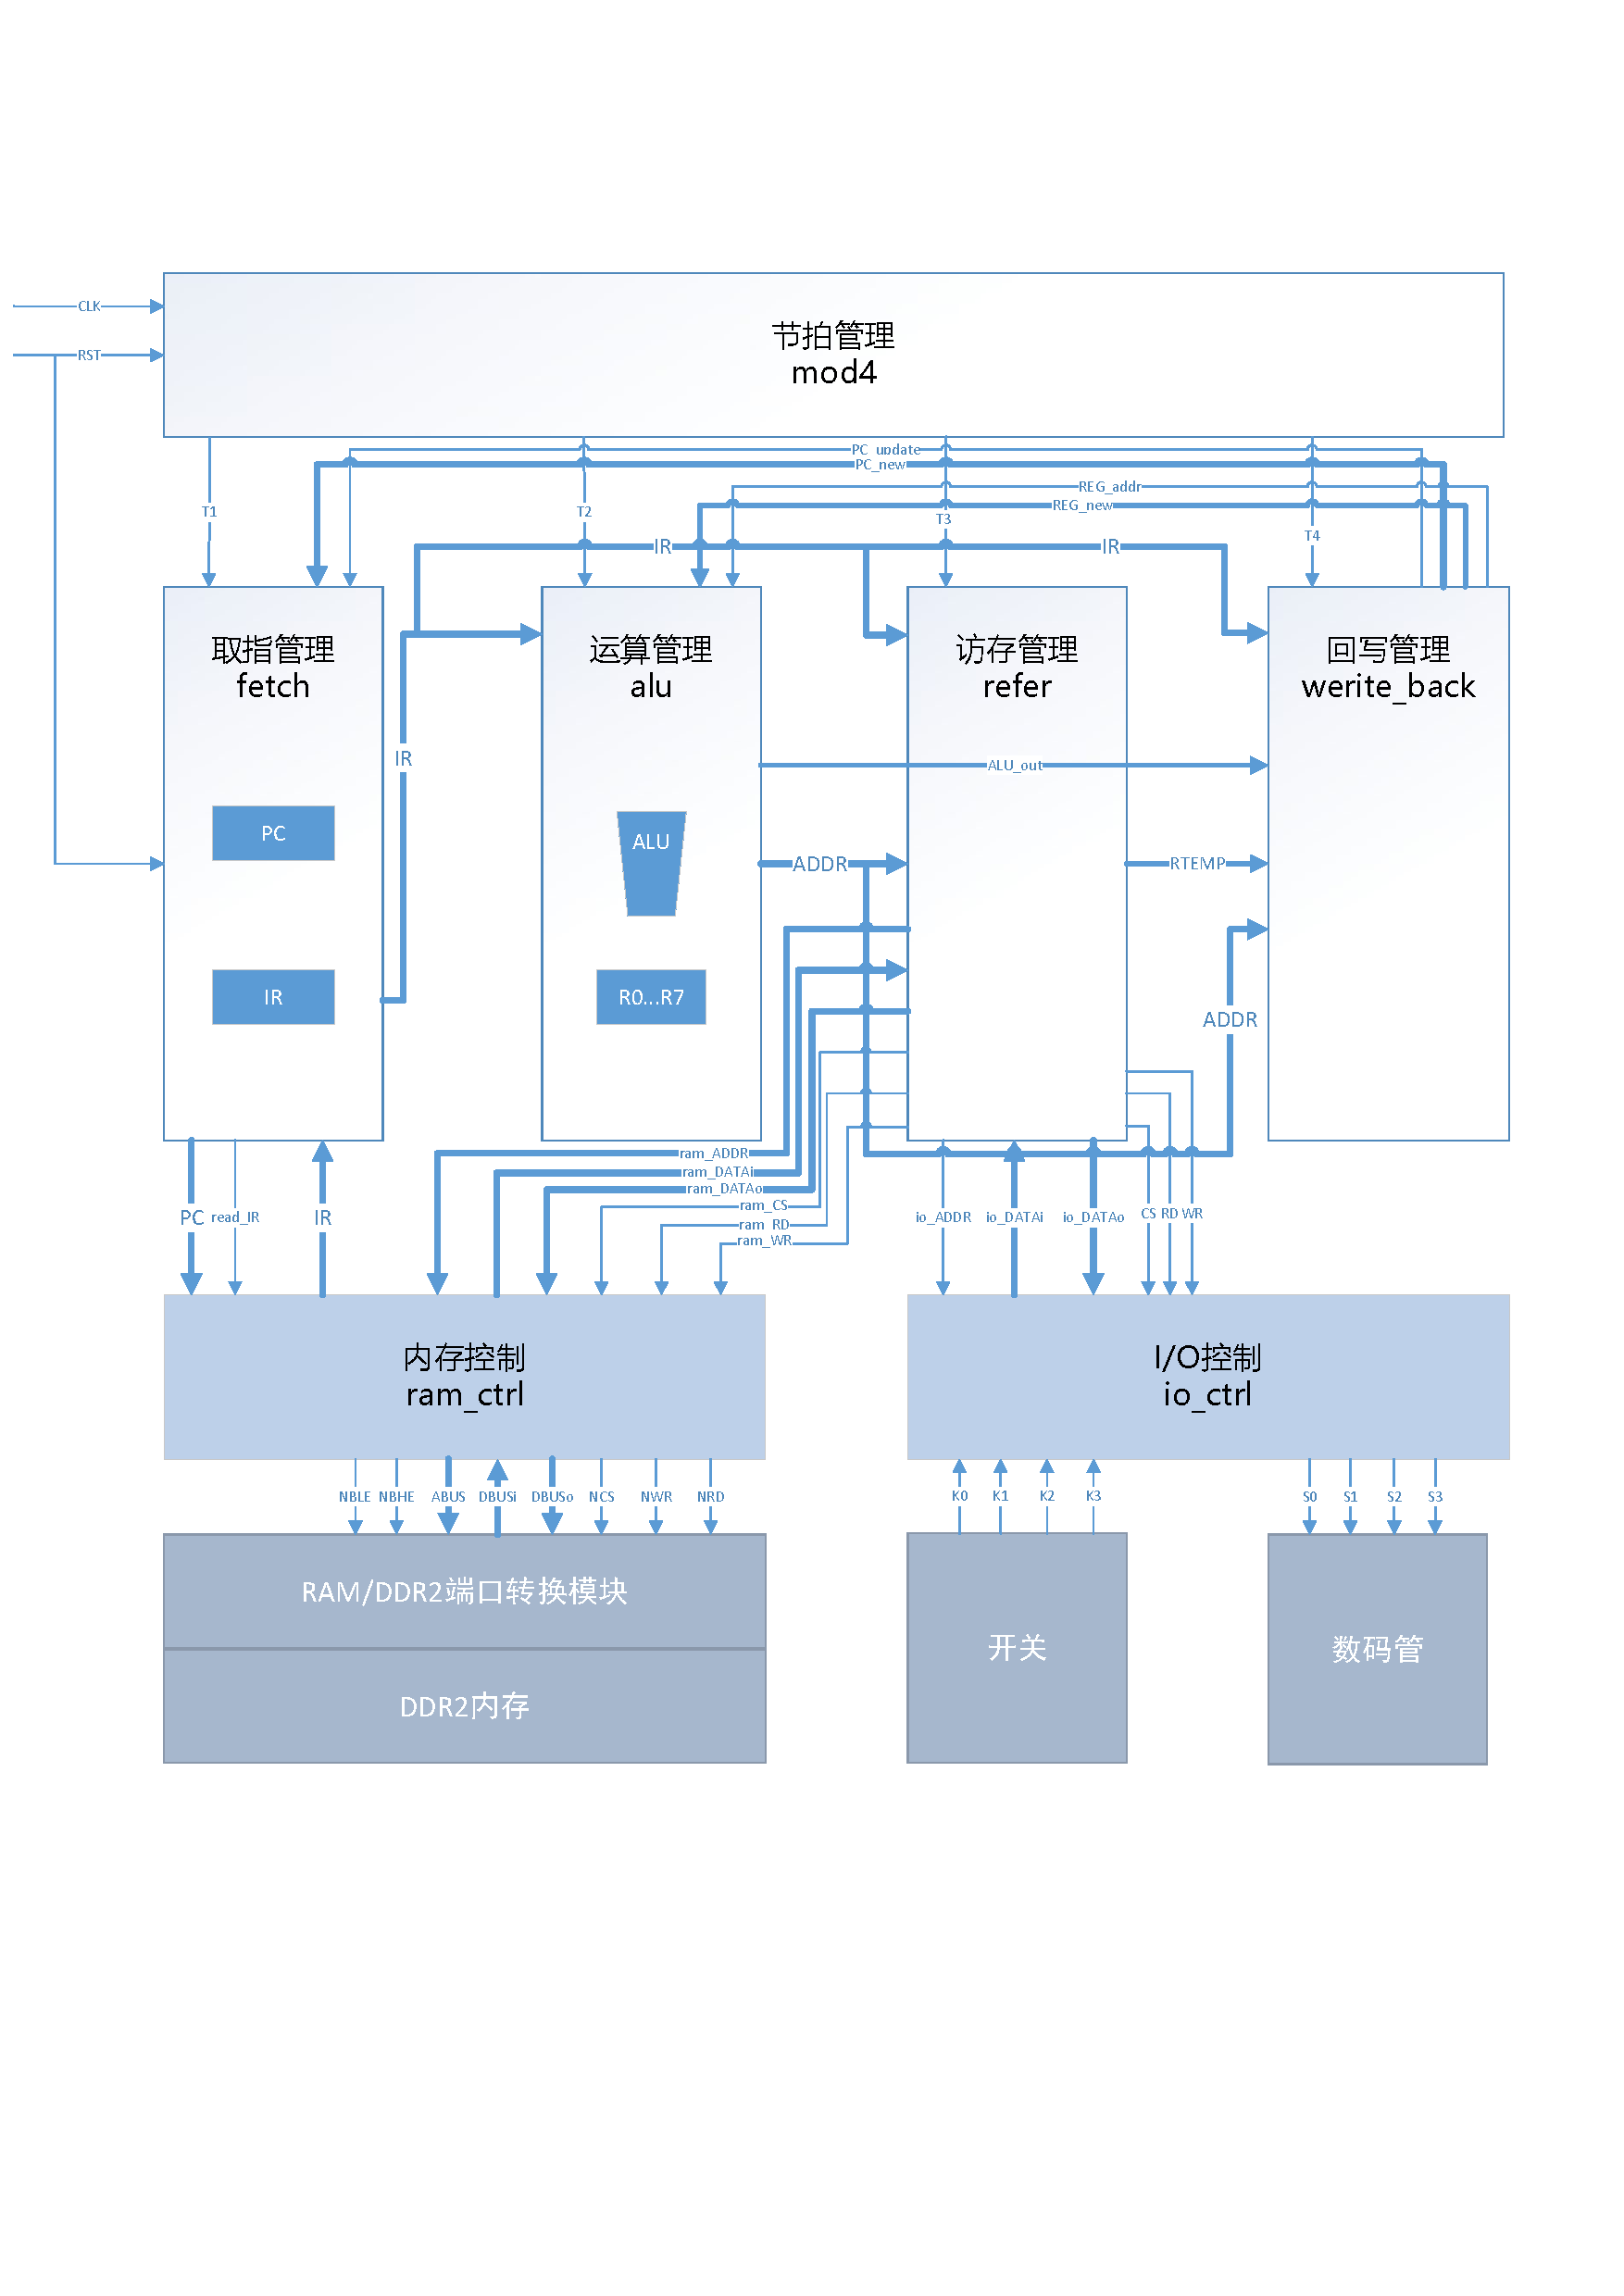
\includegraphics[width=7.6in]{figures/cpu_top.pdf}
  \caption{CPU顶端设计图}
  \label{fig:cpu_top}
\end{figure}
\thispagestyle{empty}
\restoregeometry

\chapter{各模块接口框图及定义}

{\bf 约定}:在实际编写vhdl程序时,对于每个模块,本人在输入信号前添加了''I\_''来标记,输出信号前添加了''O\_''来标记,输入输出信号前添加了''IO\_''来标记。

\section{顶端模块(cpu)}

CPU的顶端模块的端口定义如下:

\begin{table}[ht]
  \centering
  \begin{tabular}{c c c c c}
    \hline
    信号名称 & 位数 & 方向 &来源/去向 & 信号意义 \\
    \hline
    I\_CLK\_100MHZ & 1 & I & 开发板时钟 & 开发板时钟 \\
    I\_CLK & 1 & I & 开发板BTNU按钮 & 系统时钟 \\
    I\_RST & 1 & I & 开发板BTND按钮 & 复位信号(高电平有效) \\
    I\_K0, I\_K1, I\_K2, I\_K3 & 8 & I & 拨动开关 & I/O输入设备 \\
    O\_S0, O\_S0, O\_S0, O\_S0 & 8 & O & LED灯 & I/O输出设备 \\
    ddr2\_addr & 12 & O & 存储器 & 访存地址 \\
    ddr2\_ba & 3 & O & 存储器 & 内存bank选择\\
    ddr2\_ras\_n, ddr2\_ck\_p & 1 & O & 存储器 & DDR2存储器读写控制信号 \\
    ddr2\_cke, ddr2\_cs\_n & 1 & O & 存储器 & DDR2存储器读写控制信号\\
    ddr2\_ck\_n, ddr2\_odt & 1 & O & 存储器 & DDR2存储器读写控制信号\\
    ddr2\_dqs\_p, ddr2\_dqs\_n & 2 & IO & 存储器 & DDR2存储器时钟控制信号\\
    ddr2\_dm & 2 & O & 存储器 & DDR2存储器数据掩码相关 \\
    ddr2\_dq & 16 & IO & 存储器 & DDR2存储器访存数据 \\
    \hline
  \end{tabular}
  \caption{顶端模块端口定义}
  \label{tab:ports:cpu}
\end{table}

\section{节拍管理(mod4)}

节拍管理模块的端口框图如下:

\begin{figure}[H]
  \centering
  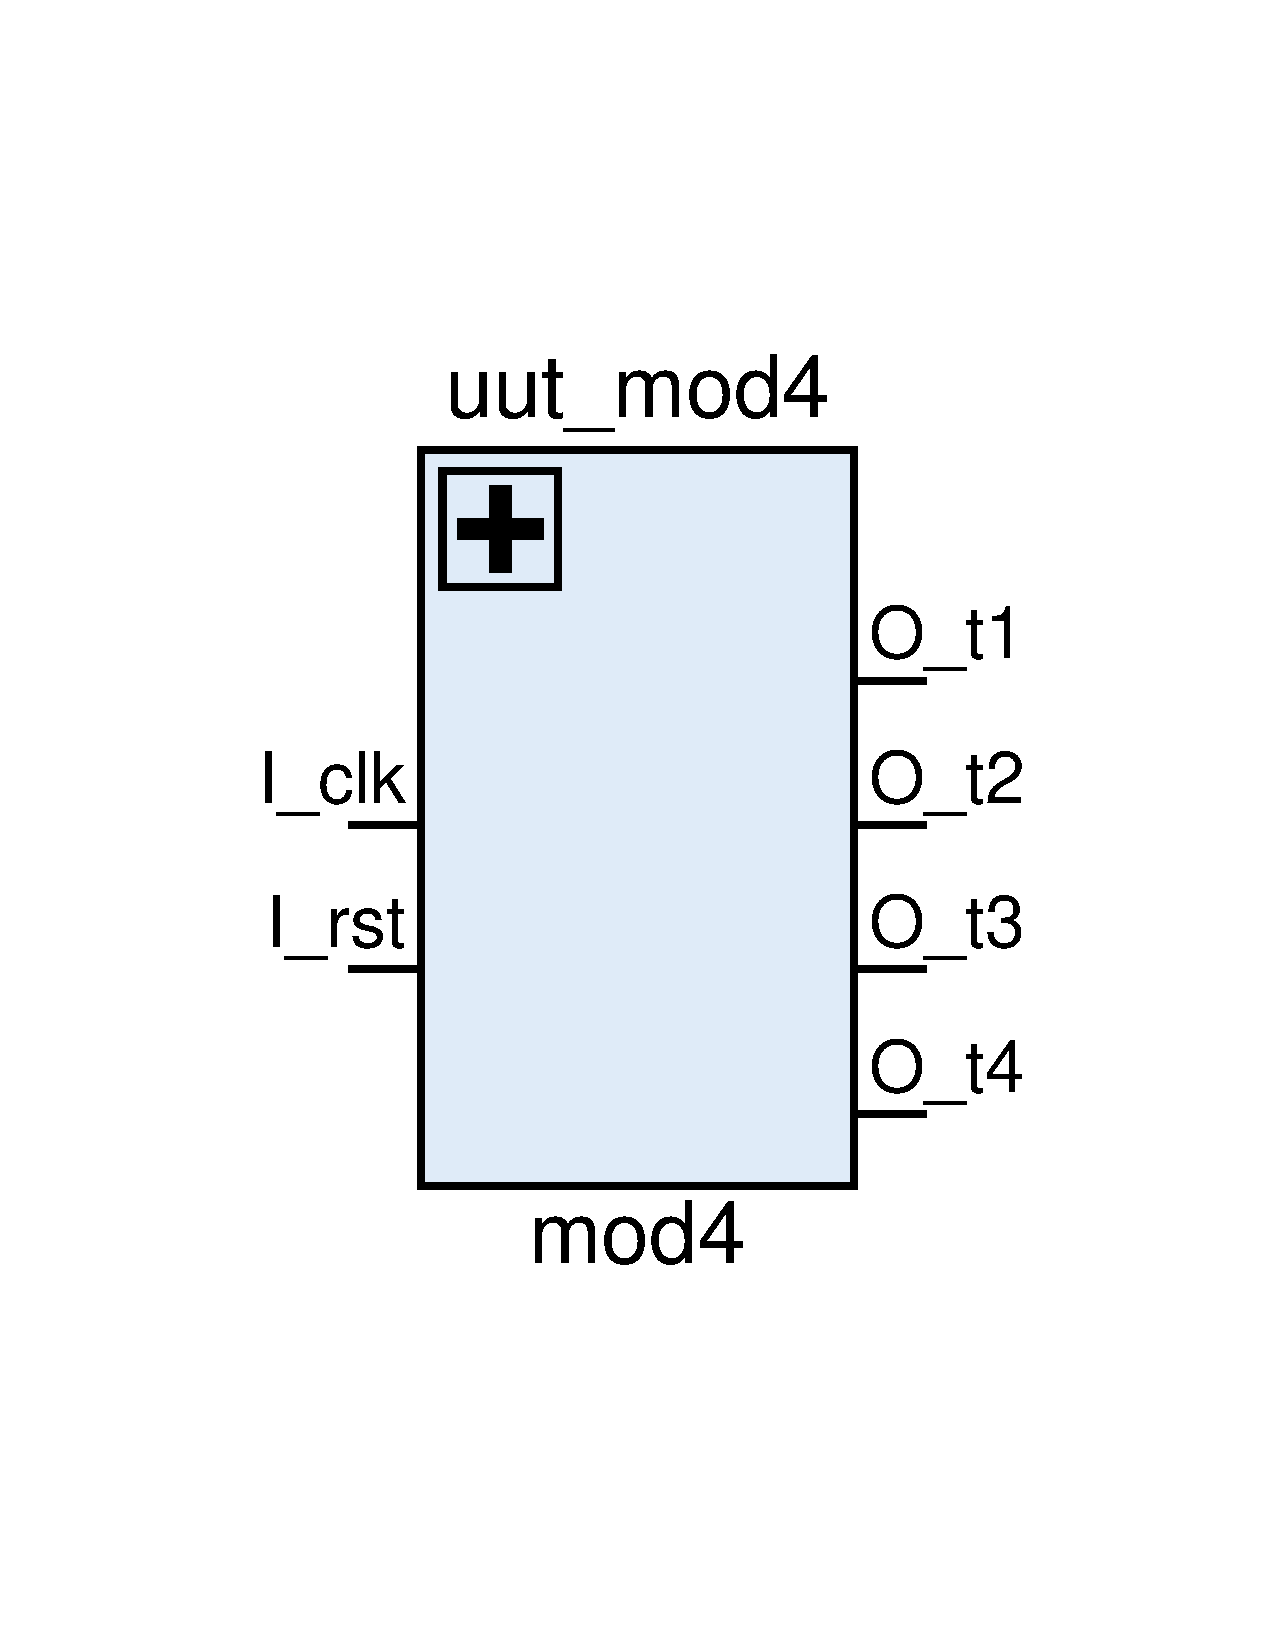
\includegraphics[width=3in]{figures/ports/mod4.pdf}
  \caption{节拍管理模块端口框图}
  \label{fig:ports:mod4}
\end{figure}

其中,各端口的定义如下:

\begin{table}[ht]
  \centering
  \begin{tabular}{c c c c c}
    \hline
    信号名称 & 位数 & 方向 & 来源/去向 & 信号意义 \\
    \hline
    I\_rst & 1 & I & 开发板BTND按钮 & 复位信号(高电平有效)\\
    I\_clk & 1 & I & 开发板BNUU按钮 & 系统时钟 \\
    O\_t1 & 1 & O & 取指管理模块 & 取指周期节拍 \\
    O\_t2 & 1 & O & 运算管理模块 & 运算周期节拍 \\
    O\_t3 & 1 & O & 访存管理模块 & 访存周期节拍 \\
    O\_t4 & 1 & O & 回写管理模块 & 回写周期节拍 \\
    \hline
  \end{tabular}
  \caption{节拍管理模块的端口定义}
  \label{tab:ports:mod4}
\end{table}

\section{取指管理(fetch)}

\begin{figure}[H]
  \centering
  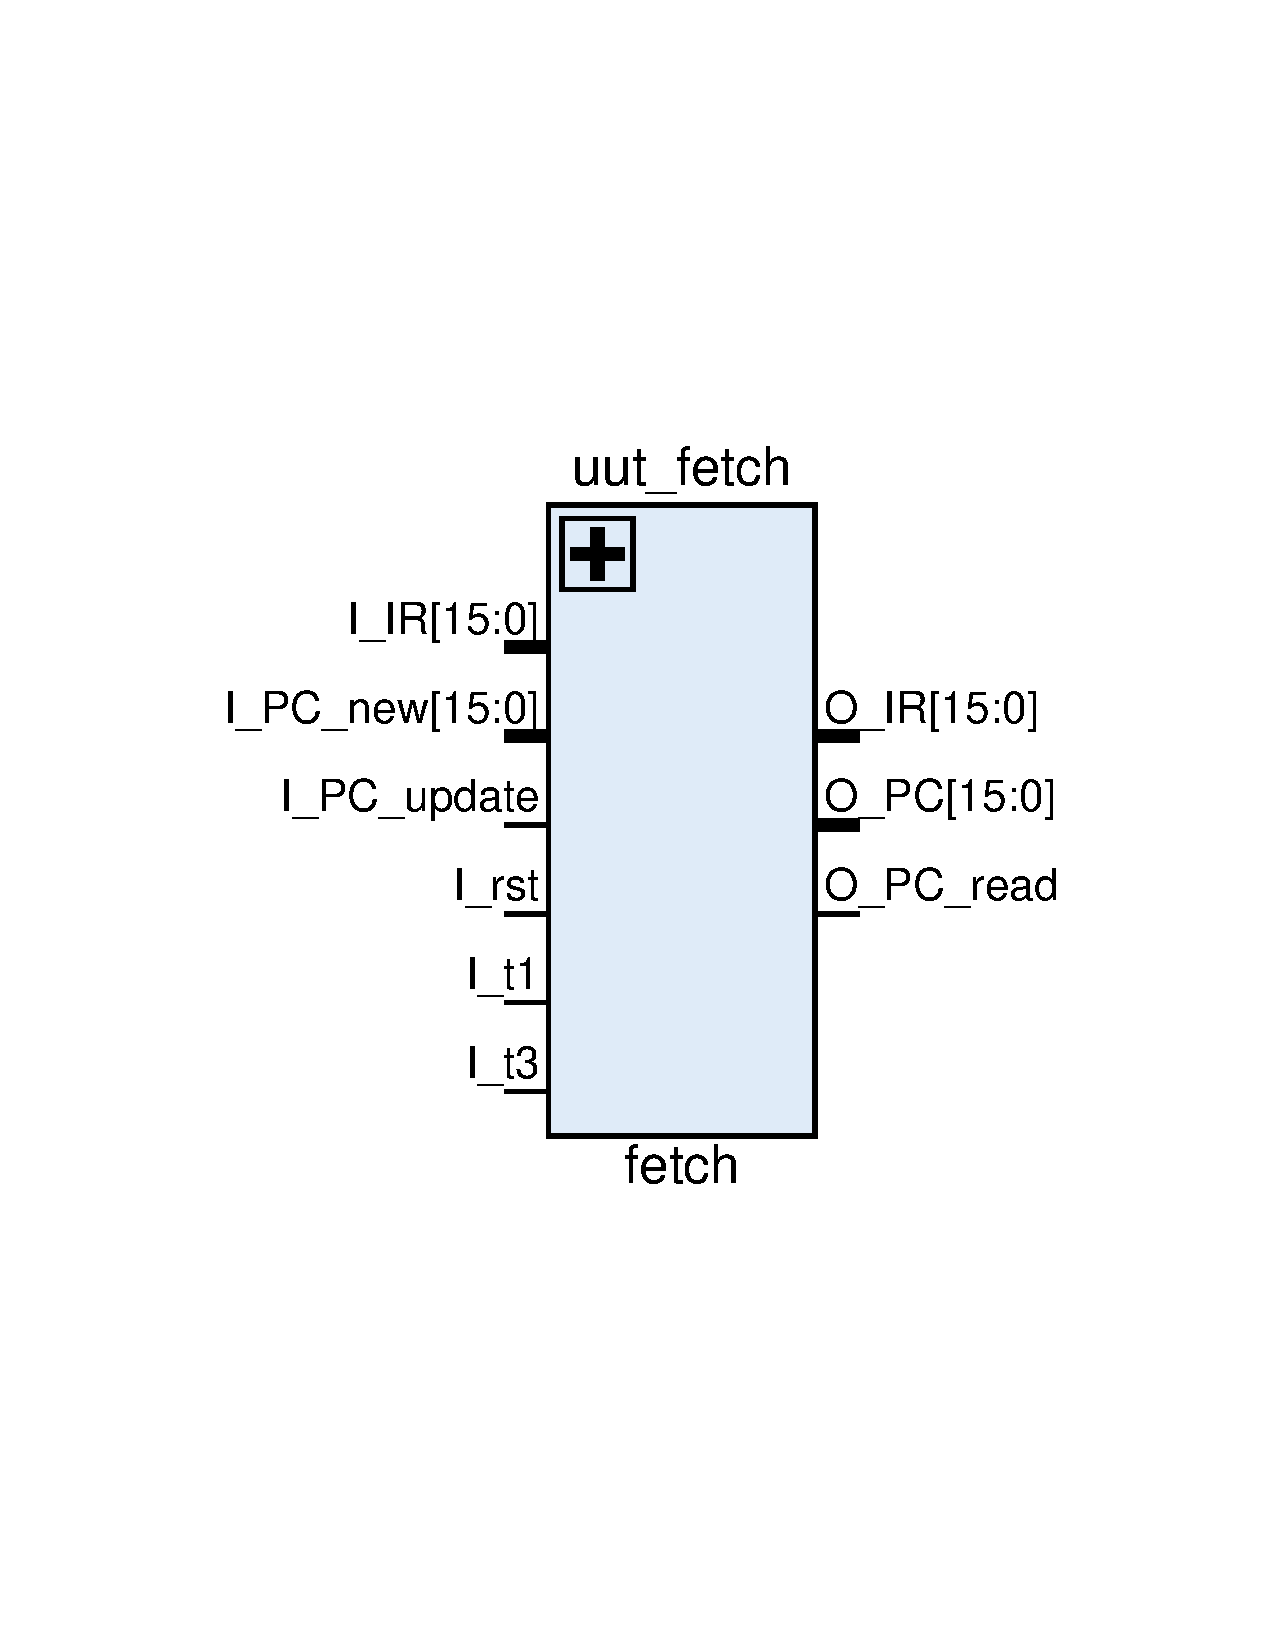
\includegraphics[width=3in]{figures/ports/fetch.pdf}
  \caption{取指管理模块端口框图}
  \label{fig:ports:fetch}
\end{figure}

\begin{table}[ht]
  \centering
  \begin{tabular}{c c c c c}
    \hline
    信号名称 & 位数 & 方向 & 来源/去向 & 信号意义 \\
    \hline
    I\_PC\_new & 16 & I & 回写管理模块 & 新的PC值 \\
    I\_PC\_update & 1 & I & 回写管理模块 & PC更新信号(高电平有效) \\
    I\_IR & 16 & I & 内存控制模块 & 读取的指令(IR) \\
    I\_rst & 1 & I & 开发板BTND按钮 & 复位信号(高电平有效) \\
    I\_t1 & 1 & I & 节拍管理模块 & 取指周期节拍 \\
    I\_t3 & 1 & I & 节拍管理模块 & 访存周期节拍 \\
    O\_IR & 16 & O & 其他三个管理模块 & 读取的指令(IR) \\
    O\_PC & 16 & O & 内存控制模块 & 当前PC值\\
    O\_PC\_read & 1 & O & 内存控制模块 & 是否从当前地址(PC)读取指令(IR)\\
    \hline
  \end{tabular}
  \caption{取指管理模块的端口定义}
  \label{tab:ports:fetch}
\end{table}

\section{运算管理(alu)}

\begin{figure}[H]
  \centering
  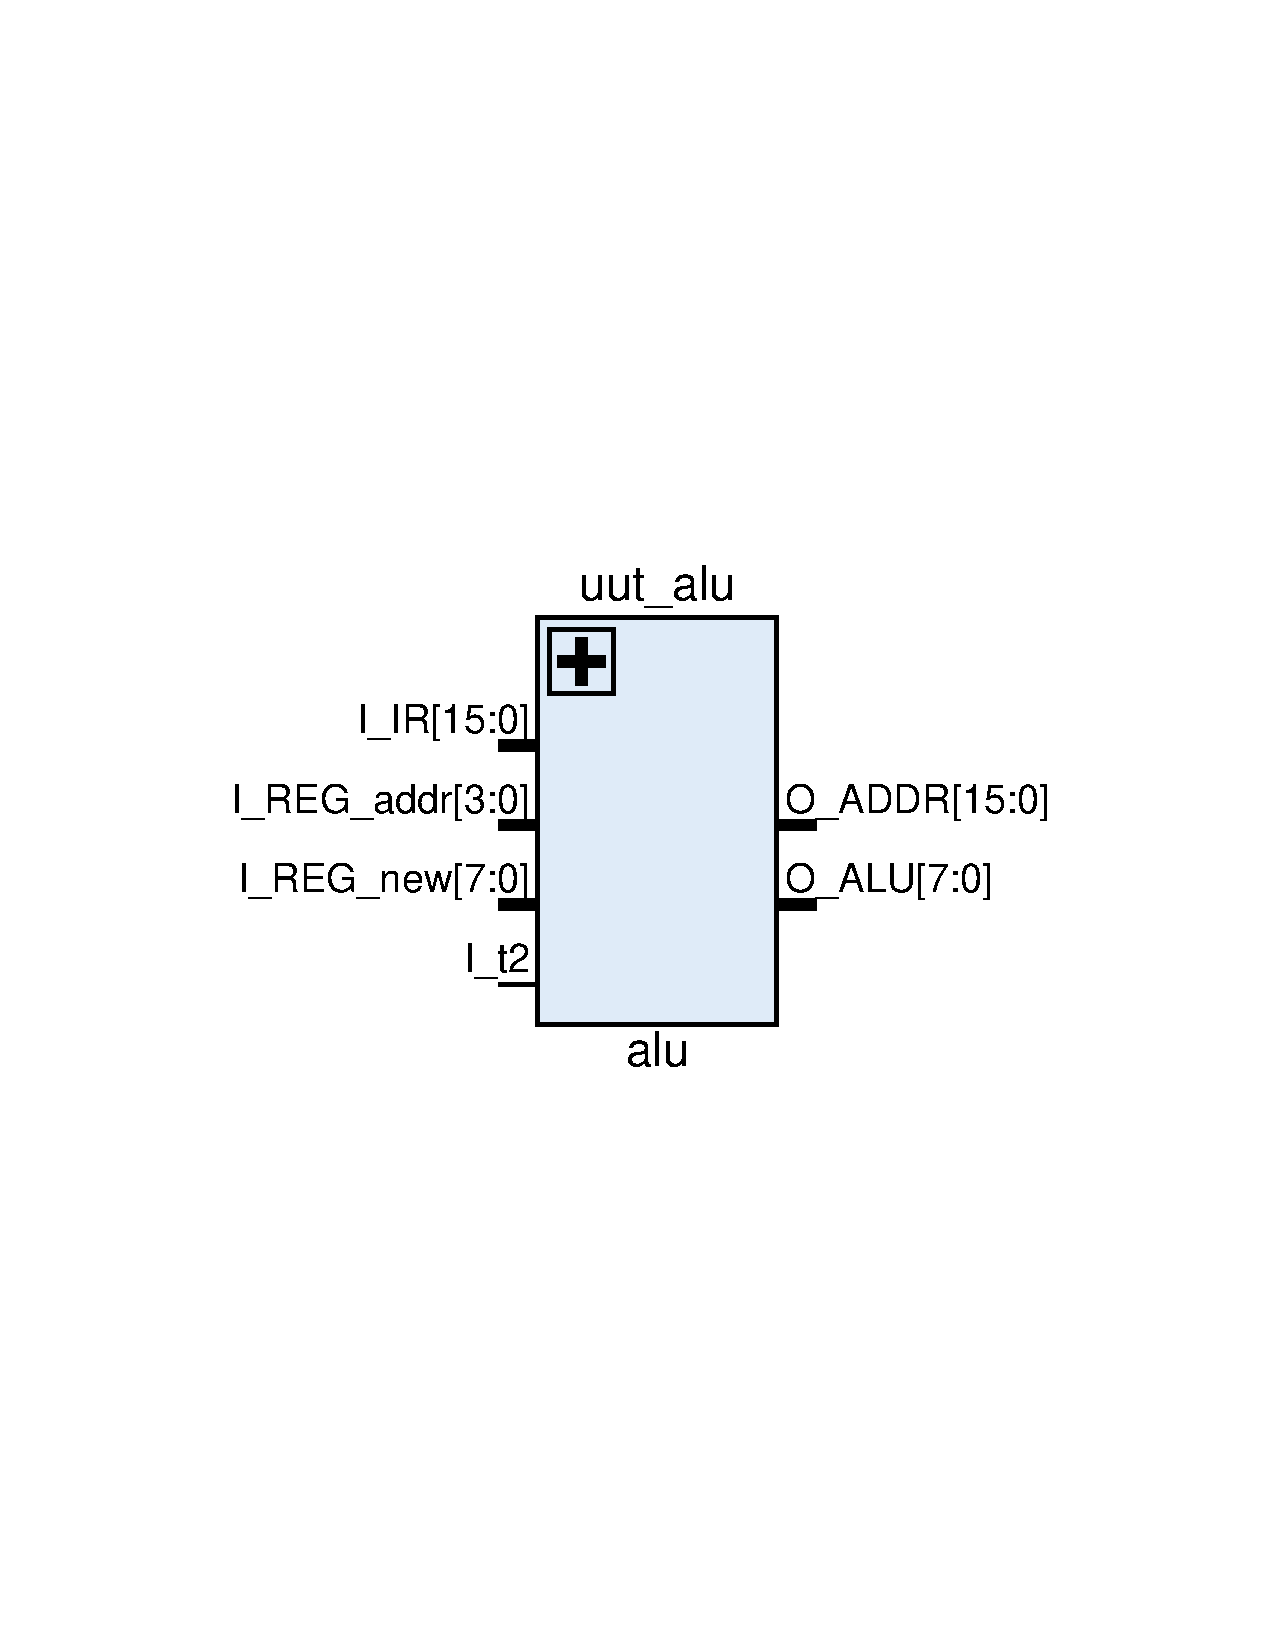
\includegraphics[width=3in]{figures/ports/alu.pdf}
  \caption{运算管理模块端口框图}
  \label{fig:ports:alu}
\end{figure}

\begin{table}[ht]
  \centering
  \begin{tabular}{c c c c c}
    \hline
    信号名称 & 位数 & 方向 & 来源/去向 & 信号意义 \\
    \hline
    I\_IR & 16 & I & 取指模块 & 当前指令(IR) \\
    I\_t2 & 1 & I & 节拍管理模块 & 运算周期节拍 \\
    I\_REG\_addr & 4 & I & 回写模块 & 需要修改的寄存器的编号 \\
    I\_REG\_new & 1 & I & 回写模块 & 需要修改的寄存器的新值 \\
    O\_ALU & 1 & I & 访存和回写模块 & 运算结果 \\
    O\_ADDR & 1 & I & 访存和回写模块 & 通过IR(7 downto 0)与R(7)计算出的地址 \\
    \hline
  \end{tabular}
  \caption{运算管理模块的端口定义}
  \label{tab:ports:alu}
\end{table}

\section{访存管理(refer)}

\begin{figure}[H]
  \centering
  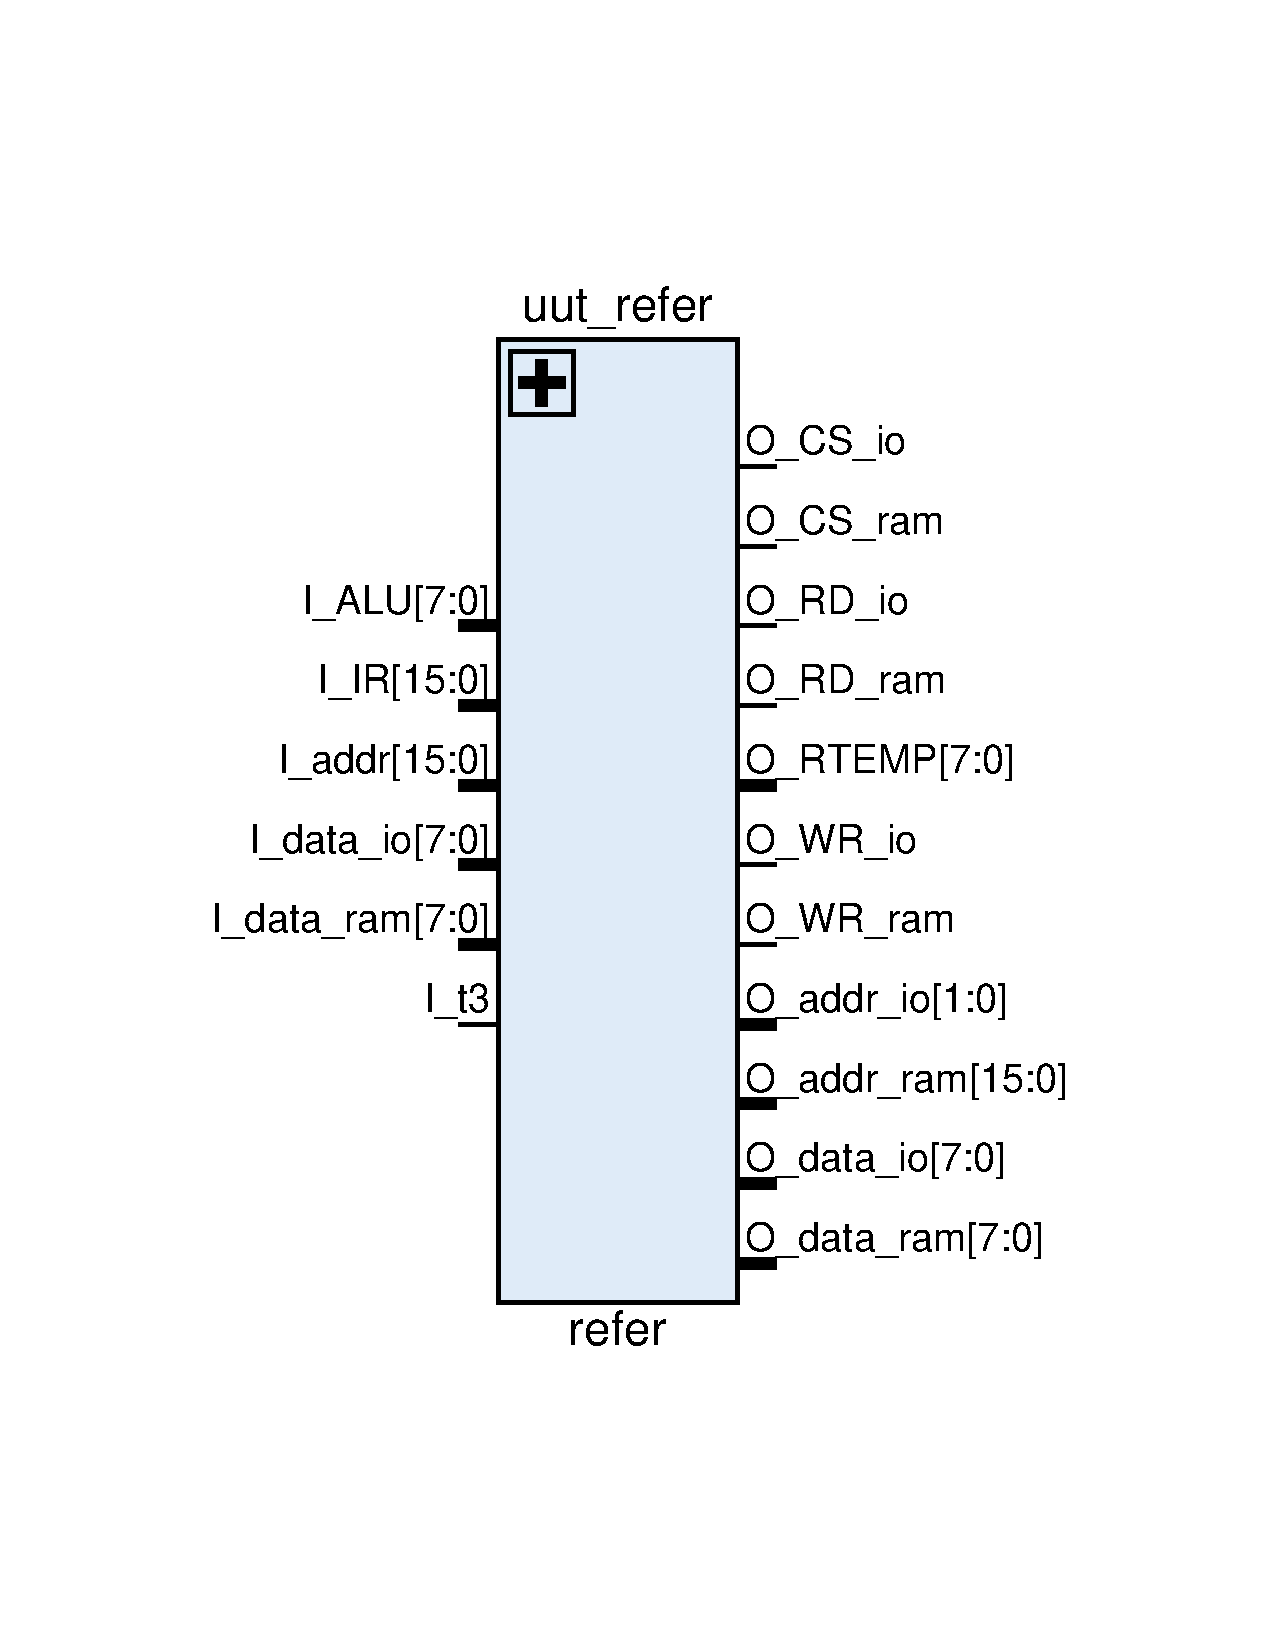
\includegraphics[width=3in]{figures/ports/refer.pdf}
  \caption{访存管理模块端口框图}
  \label{fig:ports:refer}
\end{figure}

\begin{table}[H]
  \centering
  \begin{tabular}{c c c c c}
    \hline
    信号名称 & 位数 & 方向 & 来源/去向 & 信号意义 \\
    \hline
    I\_IR & 16 & I & 取指模块 & 当前指令(IR) \\
    I\_t3 & 1 & I & 节拍管理模块 & 访存周期节拍 \\
    I\_ALU & 8 & I & 运算模块 & 运算结果 \\
    I\_ADDR & 16 & I & 运算模块 & ALU计算出的地址 \\
    O\_CS\_ram & 1 & I & 内存控制模块 & 内存控制模块使能 \\
    O\_WR\_ram & 1 & I & 内存控制模块 & 内存控制模块写 \\
    O\_RD\_ram & 1 & I & 内存控制模块 & 内存控制模块读 \\
    I\_data\_ram & 7 & I & 内存控制模块 & 内存控制模块输入数据 \\
    O\_data\_ram & 7 & I & 内存控制模块 & 内存控制模块输出数据 \\
    O\_addr\_ram & 16 & I & 内存控制模块 & 内存控制模块访存地址 \\
    O\_CS\_io & 1 & I & I/O控制模块 & I/O控制模块使能 \\
    O\_WR\_io & 1 & I & I/O控制模块 & I/O控制模块写使能 \\
    O\_RD\_io & 1 & I & I/O控制模块 & I/O控制模块读使能\\
    O\_data\_io & 8 & I & I/O控制模块 &  I/O控制模块输出数据\\
    I\_data\_io & 8 & I & I/O控制模块 &  I/O控制模块输入数据\\
    O\_addr\_io & 2 & I & I/O控制模块 &  I/O控制模块访存地址\\
    O\_RTEMP & 8 & O & 回写模块 & 从内存或者I/O端口读出的数据\\
    \hline
  \end{tabular}
  \caption{访存管理模块的端口定义}
  \label{tab:ports:refer}
\end{table}

\section{回写管理(write\_back)}

\begin{figure}[H]
  \centering
  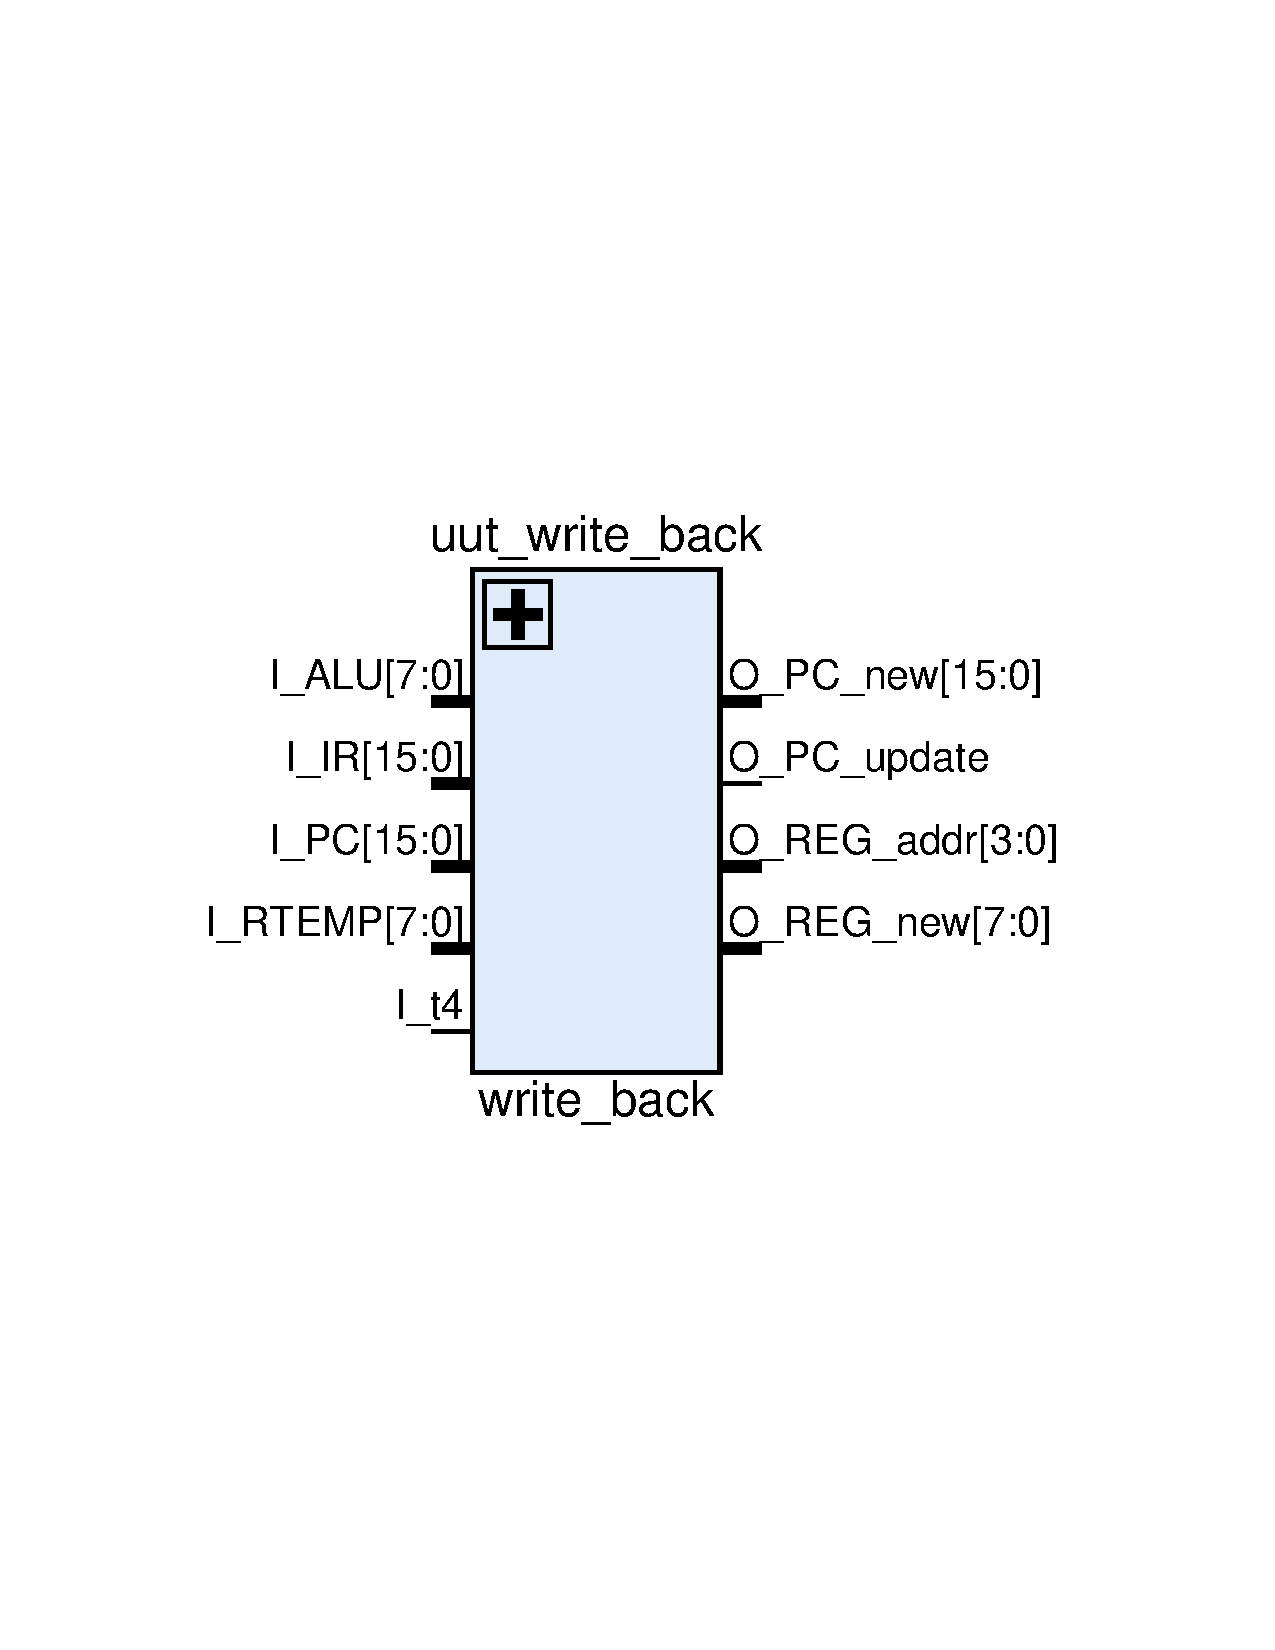
\includegraphics[width=3in]{figures/ports/write_back.pdf}
  \caption{回写管理模块端口框图}
  \label{fig:ports:write_back}
\end{figure}

\begin{table}[H]
  \centering
  \begin{tabular}{c c c c c}
    \hline
    信号名称 & 位数 & 方向 & 来源/去向 & 信号意义 \\
    \hline
    I\_IR & 16 & I & 取指模块 & 当前指令(IR) \\
    I\_t4 & 1 & I & 节拍管理模块 & 回写周期节拍 \\
    I\_RTEMP & 8 & I & 访存模块 & 访存模块从内存或者I/O端口取出的数据 \\
    I\_ADDR & 16 & I & 运算模块 & ALU算出的地址 \\
    O\_REG\_addr & 4 & O & 运算模块 & 需要改写的寄存器的编号 \\
    O\_REG\_new & 8 & O & 运算模块 & 需要改写的寄存器的新值 \\
    O\_PC\_update & 1 & O & 取指模块 & PC修改信号(高电平有效)\\
    O\_PC\_new & 16 & O & 取指模块 & PC需要修改的新值\\
    \hline
  \end{tabular}
  \caption{回写管理模块的端口定义}
  \label{tab:ports:write_back}
\end{table}

\section{内存控制(ram\_ctrl)}

\begin{figure}[H]
  \centering
  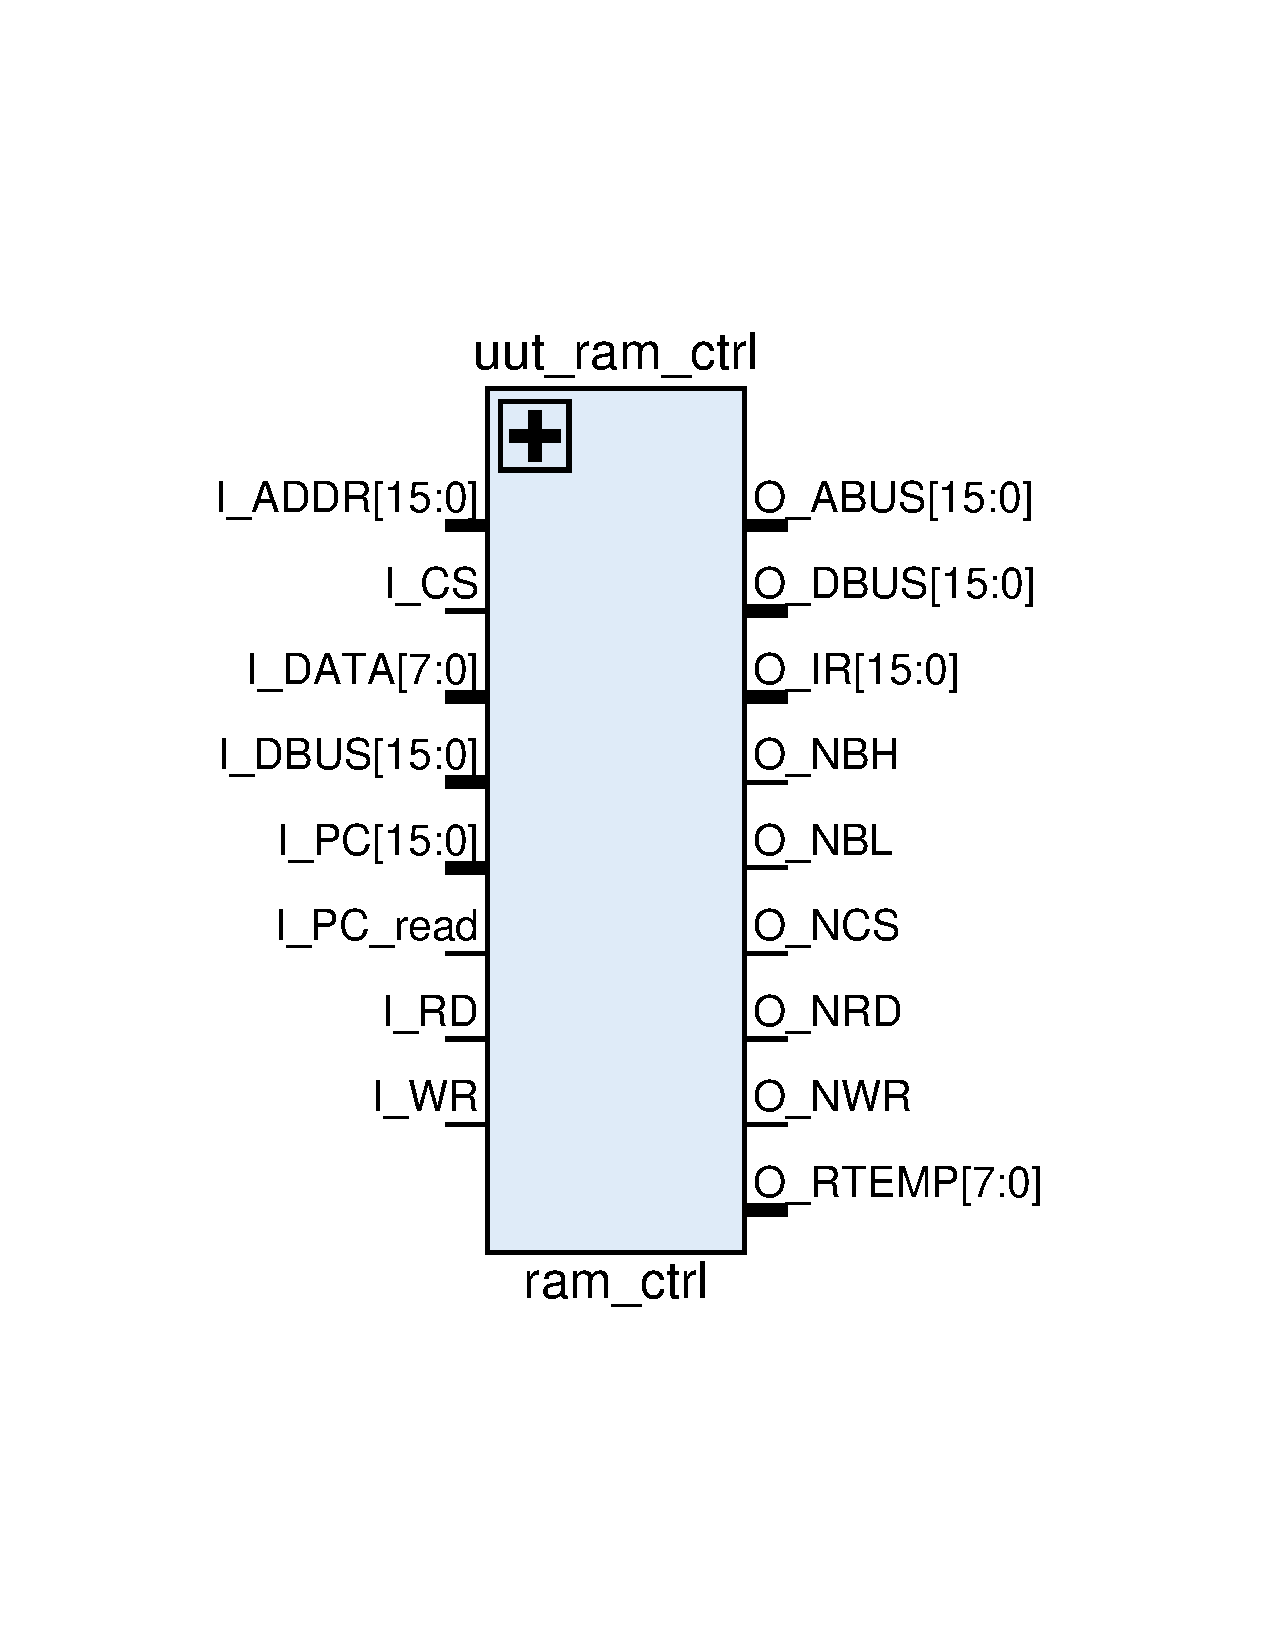
\includegraphics[width=3in]{figures/ports/ram_ctrl.pdf}
  \caption{内存控制模块端口框图}
  \label{fig:ports:ram_ctrl}
\end{figure}

\begin{table}[H]
  \centering
  \begin{tabular}{c c c c c}
    \hline
    信号名称 & 位数 & 方向 & 来源/去向 & 信号意义 \\
    \hline
    I\_PC & 16 & I & 取指模块 & 当前指令(IR) \\
    I\_PC\_read & 1 & I & 取指模块 & 从内存中读指令信号(高电平有效) \\
    O\_IR & 16 & O & 取指模块 & 从内存中读取的指令\\
    I\_CS & 1 & I & 访存管理模块 & 片选信号(高电平有效) \\
    I\_RD & 1 & I & 访存管理模块 & 读信号(高电平有效) \\
    I\_WR & 1 & I & 访存管理模块 & 写信号(高电平有效) \\
    I\_ADDR & 16 & I & 访存管理模块 & 访存地址 \\
    I\_DATA & 8 & I & 访存管理模块 & 需要往内存中写入的数据 \\
    O\_RTEMP & 8 & O & 访存管理模块 & 从内存中读取的数据 \\
    I\_NCS & 1 & I & ram/DDR2端口转换模块 & 存储器片选(低电平有效) \\
    I\_NWR & 1 & I & ram/DDR2端口转换模块 & 存储器写使能(低电平有效) \\
    I\_NRD & 1 & I & ram/DDR2端口转换模块 & 存储器读使能(低电平有效) \\
    I\_ABUS & 16 & I & ram/DDR2端口转换模块 & 地址总线 \\
    I\_DBUS & 16 & I & ram/DDR2端口转换模块 & 数据输入总线 \\
    O\_DBUS & 16 & I & ram/DDR2端口转换模块 & 数据输出总线 \\
    \hline
  \end{tabular}
  \caption{内存控制模块的端口定义}
  \label{tab:ports:ram_ctrl}
\end{table}

\section{I/O控制(io\_ctrl)}

\begin{figure}[H]
  \centering
  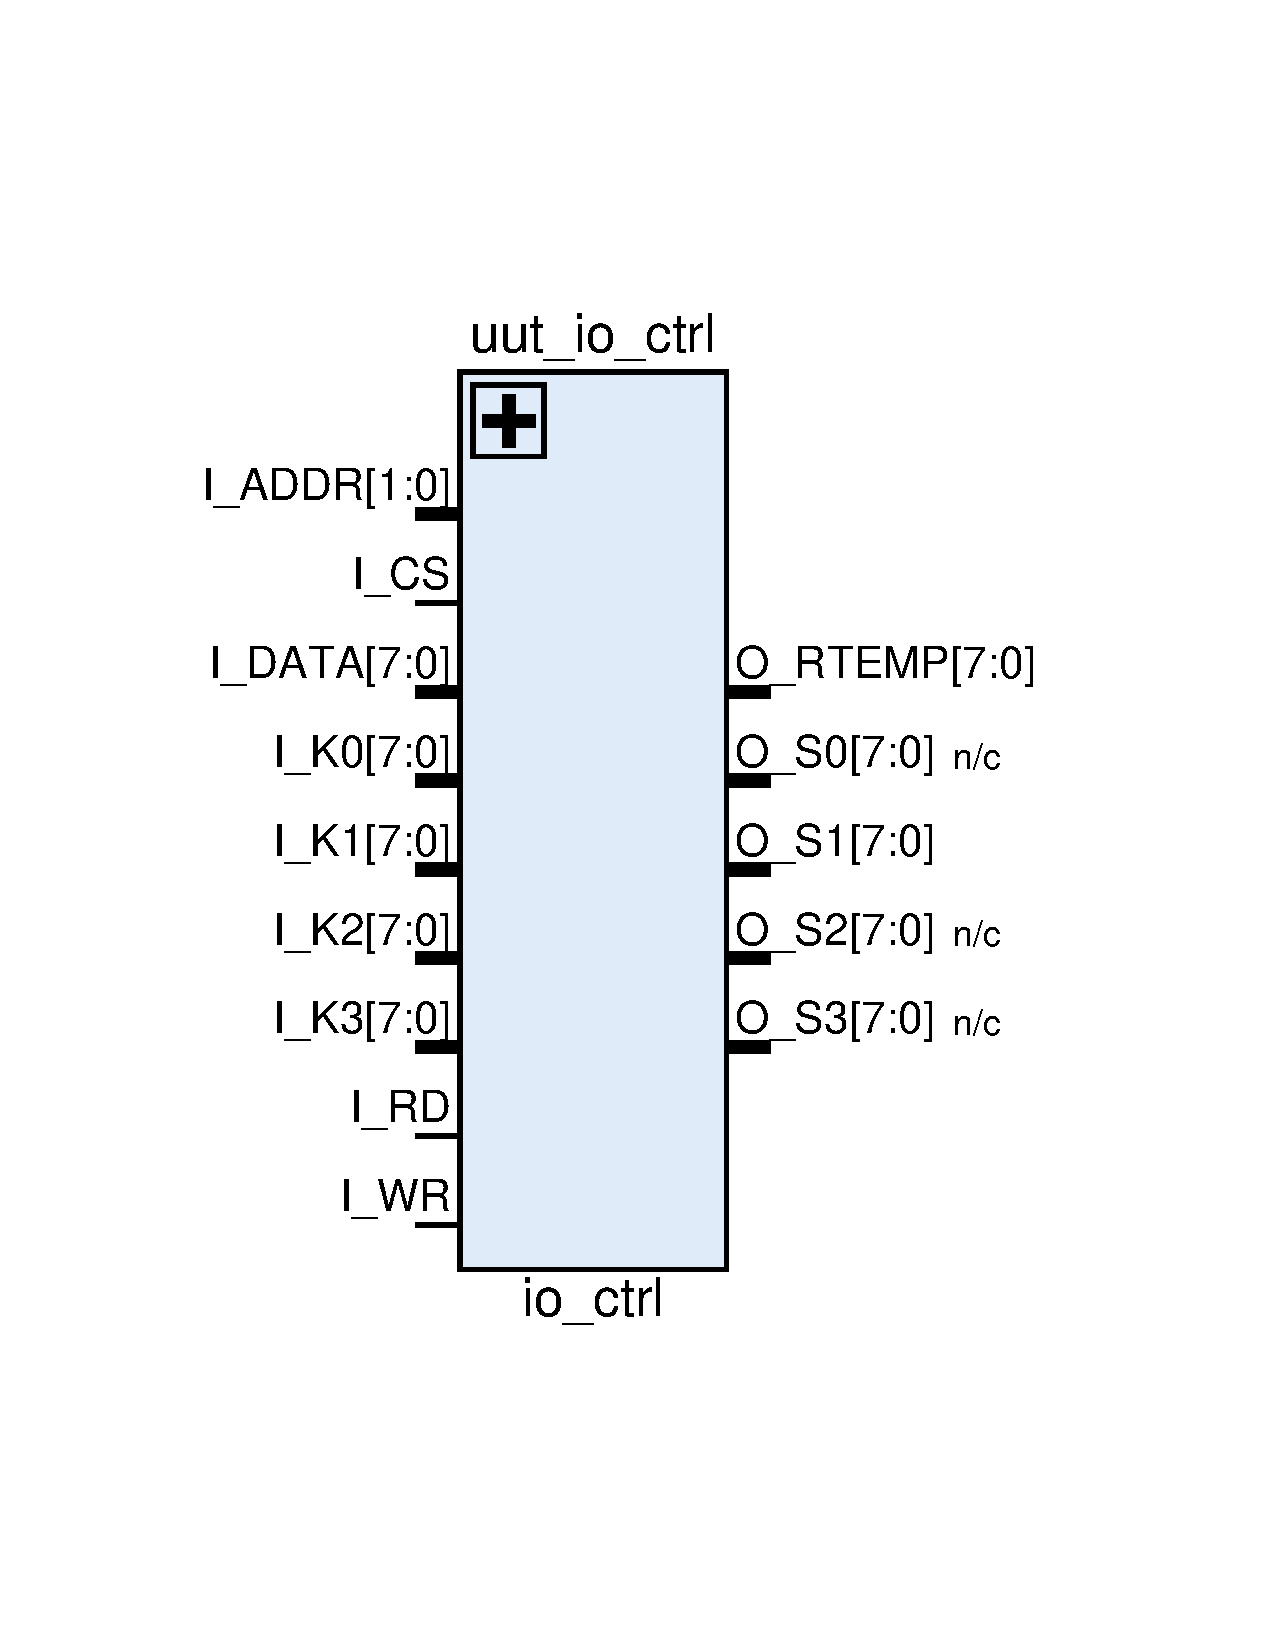
\includegraphics[width=3in]{figures/ports/io_ctrl.pdf}
  \caption{I/O控制模块端口框图}
  \label{fig:ports:ram_ctrl}
\end{figure}

\begin{table}[H]
  \centering
  \begin{tabular}{c c c c c}
    \hline
    信号名称 & 位数 & 方向 & 来源/去向 & 信号意义 \\
    \hline
    I\_CS & 1 & I & 访存管理模块 & 片选信号(高电平有效) \\
    I\_RD & 1 & I & 访存管理模块 & 读信号(高电平有效) \\
    I\_WR & 1 & I & 访存管理模块 & 写信号(高电平有效) \\
    I\_ADDR & 2 & I & 访存管理模块 & 访存地址 \\
    I\_DATA & 8 & I & 访存管理模块 & 往I/O端口中写入的数据 \\
    O\_RTEMP & 8 & O & 访存管理模块 & 从I/O端口中读取的数据 \\
    O\_S0, O\_S1, O\_S2, O\_S3 & 8 & O & led灯 & I/O输出设备\\
    I\_K0, I\_K1, I\_K2, I\_K3 & 8 & I & 开关 & I/O输入设备\\
    \hline
  \end{tabular}
  \caption{I/O控制模块的端口定义}
  \label{tab:ports:io_ctrl}
\end{table}

\section{ram/DDR2端口转换模块(ram2ddr)\protect\footnote{此模块使用的代码为Digilent公司的开源代码,可将DDR2 RAM的端口转化为Cecullar RAM的端口,以方便使用。}}

\begin{figure}[H]
  \centering
  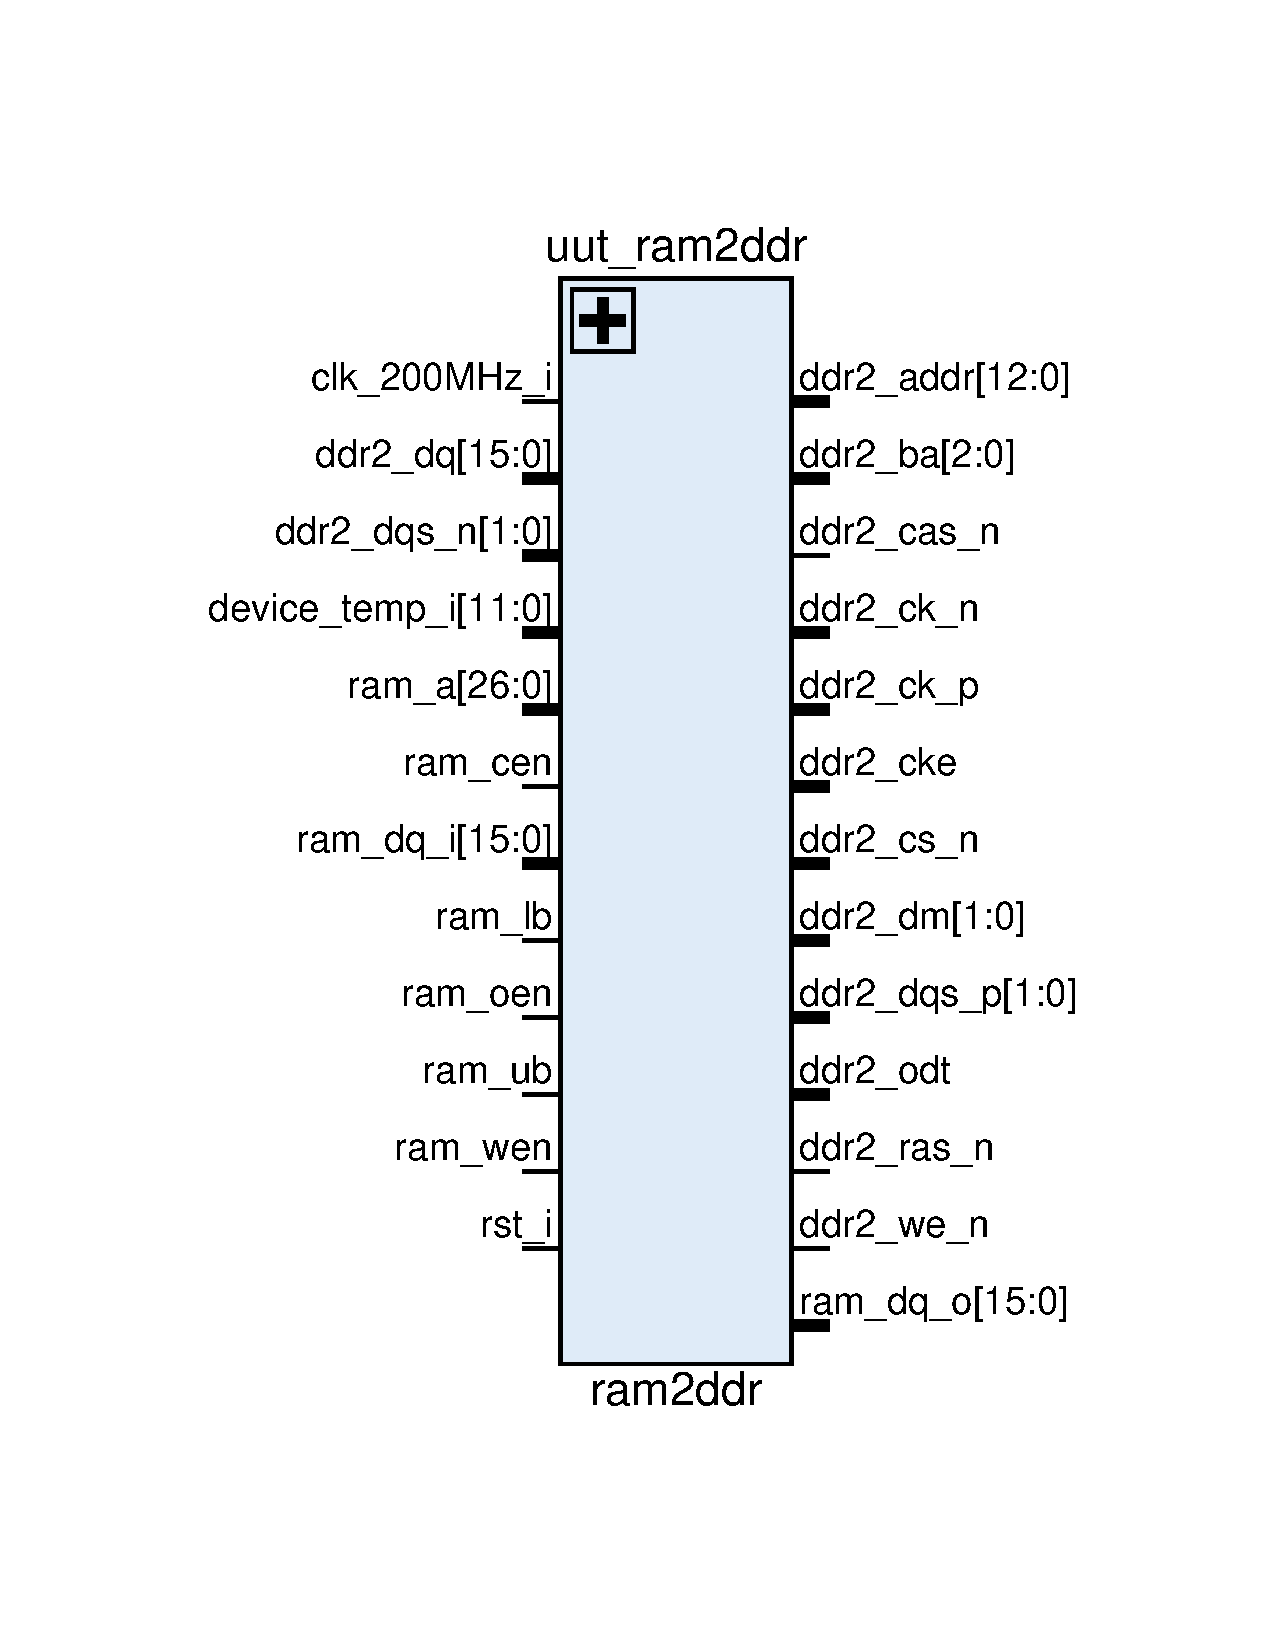
\includegraphics[width=3in]{figures/ports/ram2ddr.pdf}
  \caption{ram/DDR2端口转换模块框图}
  \label{fig:ports:ram2ddr}
\end{figure}

\begin{table}[H]
  \centering
  \begin{tabular}{c c c c c}
    \hline
    信号名称 & 位数 & 方向 & 来源/去向 & 信号意义 \\
    \hline
    clk\_200MHz\_i & 1 & I & cpu主模块 & 内存正常工作所需要的200MHz信号\\
    rst\_i & 1 & I & cpu主模块 & 内存复位信号(高电平有效)\\
    ram\_a & 27 & I & CPU主模块 & 内存访存地址\footnotemark\\
    ram\_dq\_i & 16 & I & 内存控制模块 & 写入内存的数据\\
    ram\_dq\_o & 16 & O & 内存控制模块 & 从内存中读出的数据\\
    ram\_cen & 1 & O & 内存控制模块 & 内存片选信号(低电平有效)\\
    ram\_oen & 1 & O & 内存控制模块 & 内存读信号(低电平有效)\\
    ram\_wen & 1 & O & 内存控制模块 & 内存写信号(低电平有效)\\
    ram\_ub & 1 & O & 内存控制模块 & 内存高位读写信号(低电平有效)\\
    ram\_lb & 1 & O & 内存控制模块 & 内存低位读写信号(低电平有效)\\
    ddr2\_addr & 12 & O & 存储器 & 访存地址 \\
    ddr2\_ba & 3 & O & 存储器 & 内存bank选择\\
    ddr2\_ras\_n, ddr2\_ck\_p & 1 & O & 存储器 & DDR2存储器读写控制信号 \\
    ddr2\_cke, ddr2\_cs\_n & 1 & O & 存储器 & DDR2存储器读写控制信号\\
    ddr2\_ck\_n, ddr2\_odt & 1 & O & 存储器 & DDR2存储器读写控制信号\\
    ddr2\_dqs\_p, ddr2\_dqs\_n & 2 & IO & 存储器 & DDR2存储器时钟控制信号\\
    ddr2\_dm & 2 & O & 存储器 & DDR2存储器数据掩码相关 \\
    ddr2\_dq & 16 & IO & 存储器 & DDR2存储器访存数据 \\
    \hline
  \end{tabular}
  \caption{RAM/DDR2端口转换模块的端口定义}
  \label{tab:ports:ram2ddr}
\end{table}
\footnotetext{由于本CPU使用的地址总线宽度为16位,因此本人在设计时,将地址总线高位补'0'且末位补'0'(因为该DDR2内存按字节访问)形成对DDR2内存进行访存的地址。}

\chapter{软件仿真测试}

\section{顶端模块仿真测试}

\subsection{测试方案}

在测试顶端模块时,本人使用了12条指令进行测试。12条指令分别为

\begin{enumerate}[1.]
\item JMP 2
\item JZ R0, 5
\item MVI R0, 1
\item JZ R0, 2
\item MVI R7, 7
\item ADD R0, R7
\item SUB R0, R7
\item MOV R1, R0
\item STA R0, 0c
\item LDA R2, 0c
\item OUT R2, 1
\item IN R3, 01
\end{enumerate}

\subsection{测试波形}

测试结果如图\ref{fig:wave:cpu0},图\ref{fig:wave:cpu1}以及图\ref{fig:wave:cpu2},可以看出其符合期望。

\newgeometry{left=0.3cm, right=0.3cm, top=0.3cm}
\begin{figure}[H]
  \centering
  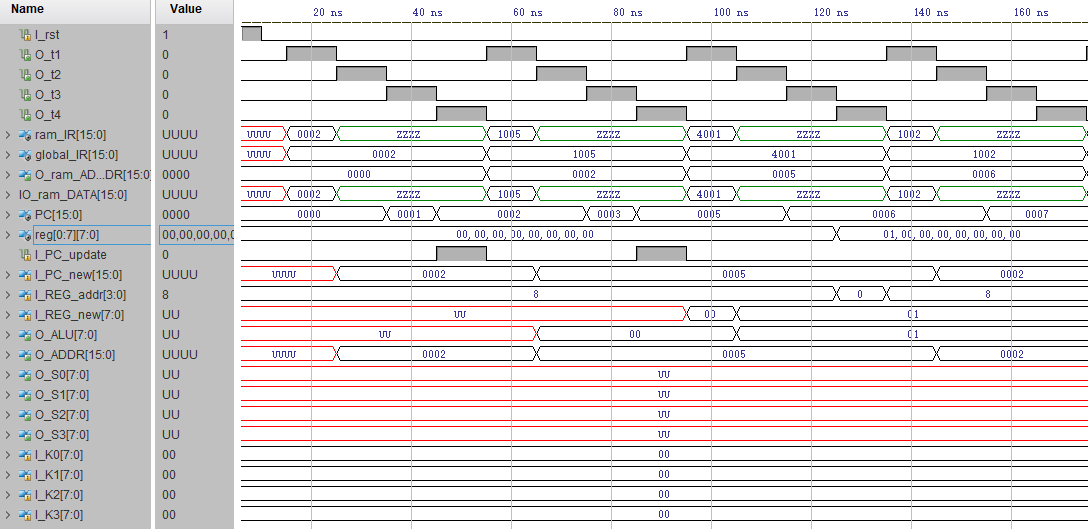
\includegraphics[width=7in]{figures/waveforms/cpu0.png}
  \caption{顶端模块仿真波形图1}
  \label{fig:wave:cpu0}
\end{figure}

\begin{figure}[H]
  \centering
  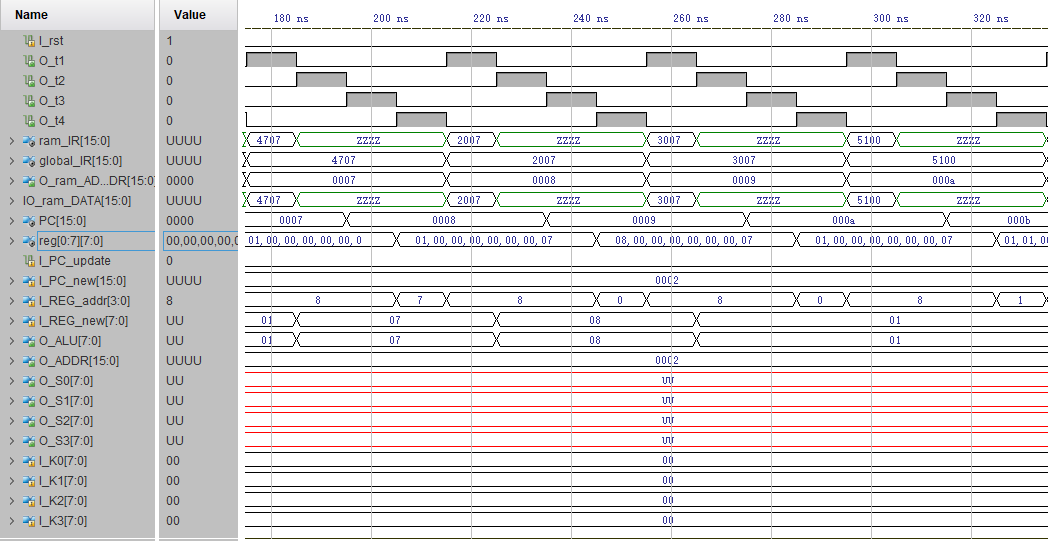
\includegraphics[width=7in]{figures/waveforms/cpu1.png}
  \caption{顶端模块仿真波形图2}
  \label{fig:wave:cpu1}
\end{figure}

\begin{figure}[H]
  \centering
  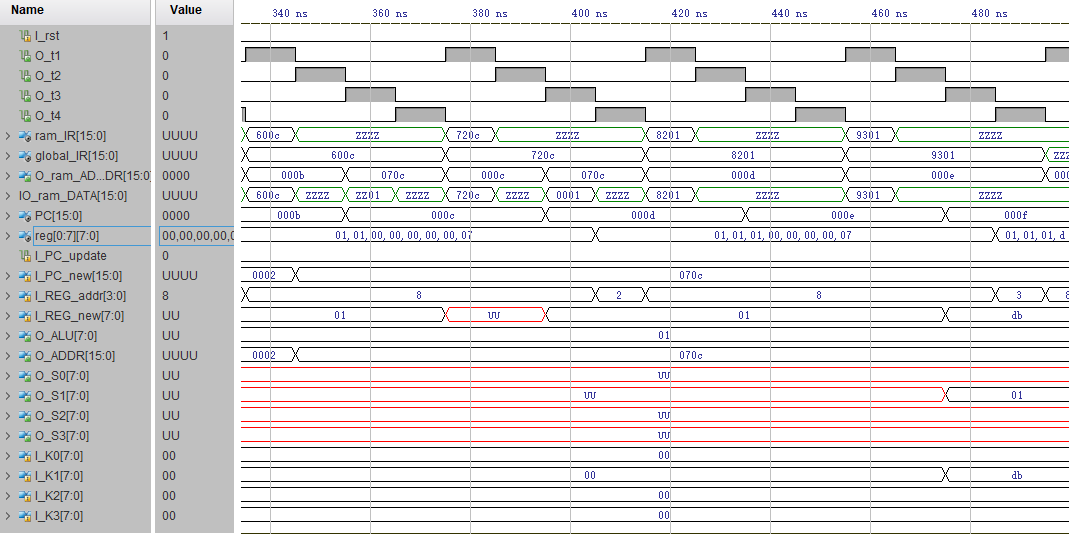
\includegraphics[width=7in]{figures/waveforms/cpu2.png}
  \caption{顶端模块仿真波形图3}
  \label{fig:wave:cpu2}
\end{figure}
\restoregeometry

\section{节拍管理模块}

\subsection{测试波形}
\begin{figure}[H]
  \centering
  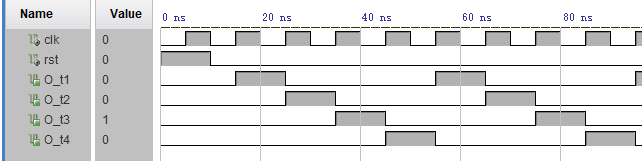
\includegraphics[width=6in]{figures/waveforms/mod4.png}
  \caption{节拍管理模块仿真波形图}
  \label{fig:wave:mod4}
\end{figure}

\section{取指管理模块}

\subsection{测试方案}

测试方案如下:
\begin{enumerate}[1.]
\item 令PC在t3自加1,此时PC=0x0001
\item 令PC\_update='1'且PC\_new=0x0005,此时PC被修改为0x0005
\item 令PC\_update保持为'0',此时PC将不断自加1
\end{enumerate}

\subsection{测试波形}

\newgeometry{left=0.3cm, right=0.3cm}
\begin{figure}[H]
  \centering
  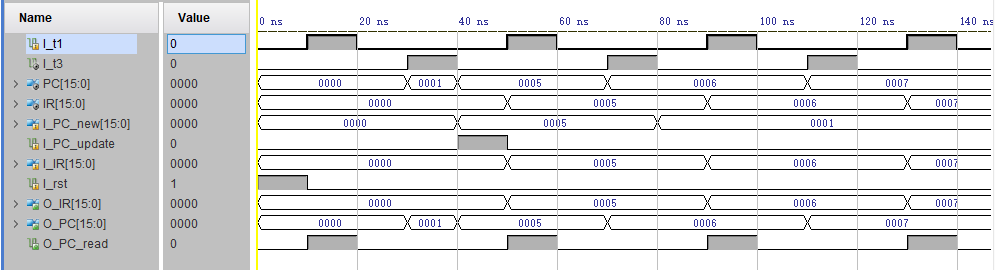
\includegraphics[width=7in]{figures/waveforms/fetch.png}
  \caption{取指管理模块仿真波形图}
  \label{fig:wave:fetch}
\end{figure}
\restoregeometry

\section{运算管理模块}

\subsection{测试方案}

在测试运算管理模块时,本人将R0初始化为1,R1初始化为2,R7初始化为5。并使用了十条指令,分别进行了模拟,十条指令为:
\begin{enumerate}[1.]
\item JMP 0xac
\item JZ R0, 0xdb
\item ADD R0, R1
\item SUB R0, R1
\item MVI R0, 0xdb
\item MOV R2, R0
\item STA R0, 0x00
\item LDA R1, 0x00
\item OUT R0, 0
\item IN R1, 0
\end{enumerate}

\subsection{测试波形}

\begin{figure}[H]
  \centering
  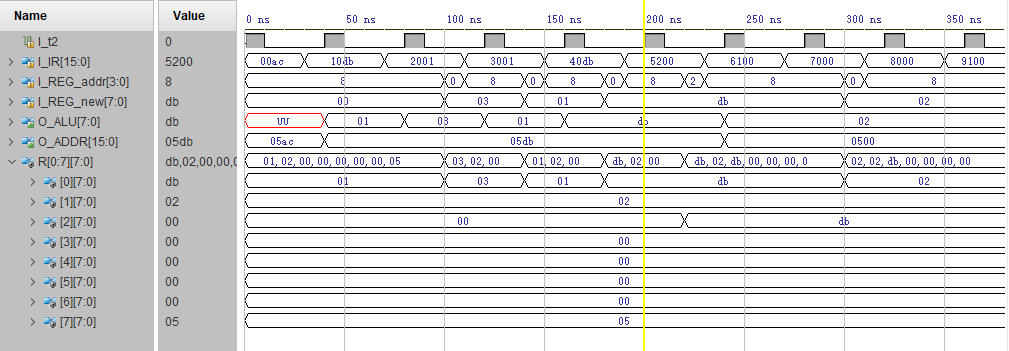
\includegraphics[width=6in]{figures/waveforms/alu.png}
  \caption{运算管理模块仿真波形图}
  \label{fig:wave:alu}
\end{figure}


\section{访存管理模块}

\subsection{测试方案}

使用了4条指令来测试,四条指令分别为:
\begin{enumerate}[1.]
\item STA R0, 0xac
\item LDA R0, 0xdb
\item OUT R0, 3
\item IN R0, 1
\end{enumerate}

\subsection{测试波形}

\begin{figure}[H]
  \centering
  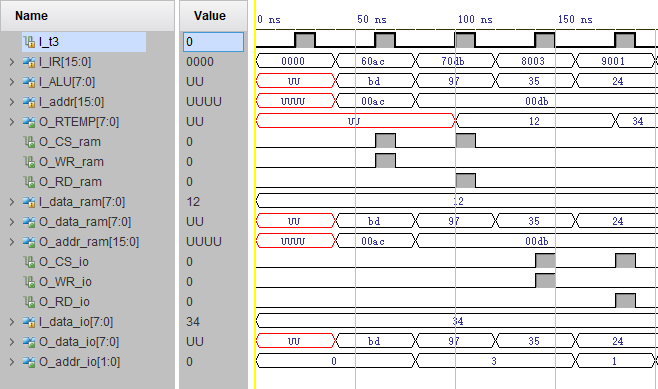
\includegraphics[width=5in]{figures/waveforms/refer.png}
  \caption{访存管理模块仿真波形图}
  \label{fig:wave:refer}
\end{figure}

\section{回写管理模块}

\subsection{测试方案}

使用了四条指令,五种情况。五种情况分别为:
\begin{enumerate}[1.]
\item JMP 0x00
\item JZ R0, 0x00(R0=0x01)
\item JZ R0, 0x00(R0=0x00)
\item ADD R0, R0
\item LDA R0, 0
\end{enumerate}

\subsection{测试波形}

\begin{figure}[H]
  \centering
  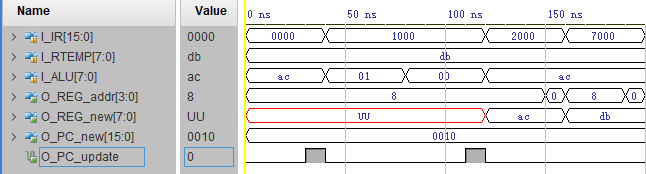
\includegraphics[width=5in]{figures/waveforms/write_back.png}
  \caption{回写管理模块仿真波形图}
  \label{fig:wave:write_back}
\end{figure}

\section{内存控制模块}

\subsection{测试方案}

令PC恒等于0xac,测试方案如下:
\begin{enumerate}[1.]
\item I\_PC\_read = '1'
\item I\_PC\_read = '0' 且 I\_CS = '0'
\item I\_CS = '1' 且 I\_RD = '1'
\item I\_CS = '1' 且 I\_WR = '1'
\end{enumerate}

\subsection{测试波形}

\begin{figure}[H]
  \centering
  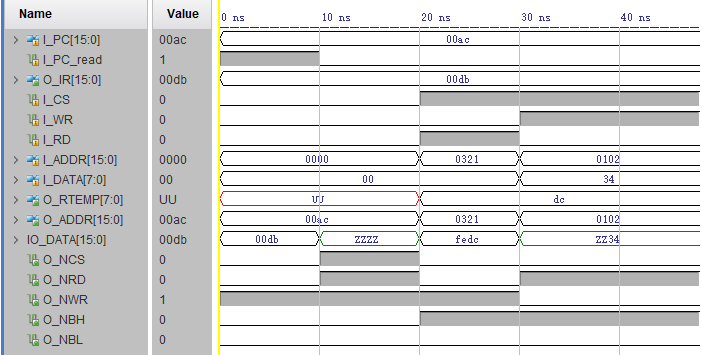
\includegraphics[width=5in]{figures/waveforms/ram_ctrl.png}
  \caption{内存控制模块仿真波形图}
  \label{fig:wave:ram_ctrl}
\end{figure}

\section{I/O控制模块}

\subsection{测试方案}

测试方案如下:
\begin{enumerate}[1.]
\item CS = '1' 且 RD = '1'(尝试两个地址)
\item CS = '1' 且 WR = '1'(尝试两个地址)
\end{enumerate}

\subsection{测试波形}

\begin{figure}[H]
  \centering
  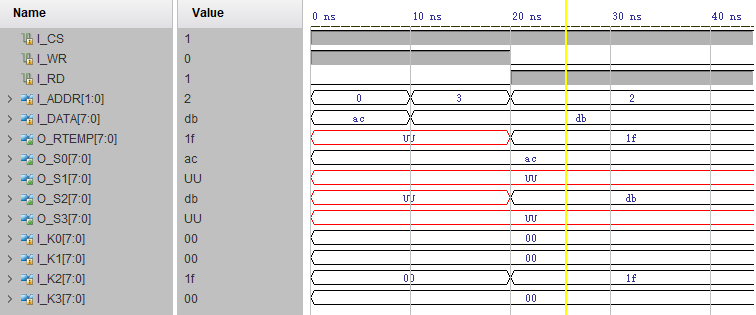
\includegraphics[width=5in]{figures/waveforms/io_ctrl.png}
  \caption{I/O控制模块仿真波形图}
  \label{fig:wave:io_ctrl}
\end{figure}

\chapter{CPU下载测试(使用Nexys 4 DDR FPGA)}

在使用CPU下载测试时,由于Nexys 4 DDR FPGA只有16个LED灯和16个开关,所以我将左边的8个开关记为K1,左边的8个LED灯记为S1。

右边的8个LED灯用来提示系统状态,从右往左依次代表:t1,t2,t3,t4,ram\_CS,ram\_RD,ram\_WR,PC\_update。

最右边的开关在开启时(向上拨),左边的4位七段数码管显示的是地址总线,右边的4位七段数码管显示的是数据总线;而当最右边的开关向下拨时,左边的2位七段数码管显示的是ALU\_out,旁边的两位七段数码管显示的是PC的低8位,最右边的4位七段数码管显示的是IR的值。

\section{指令1:JMP 0x01(地址0x0000)}


\begin{figure}[H]
  \centering
  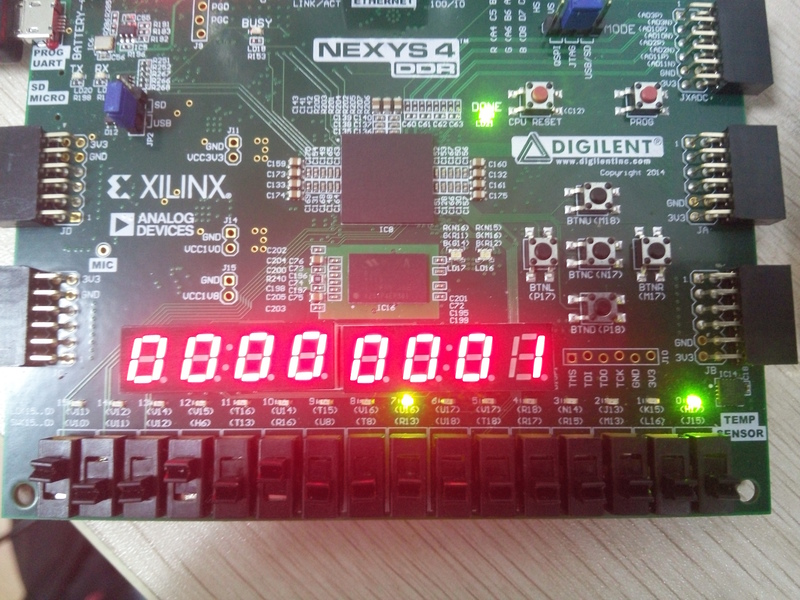
\includegraphics[width=5in]{figures/download/00.jpg}
  \caption{指令1在t1时}
  \label{fig:down:00}
\end{figure}

由图\ref{fig:down:00}可以看出,在t1时,PC=0x0000,IR=0x0001。

\begin{figure}[H]
  \centering
  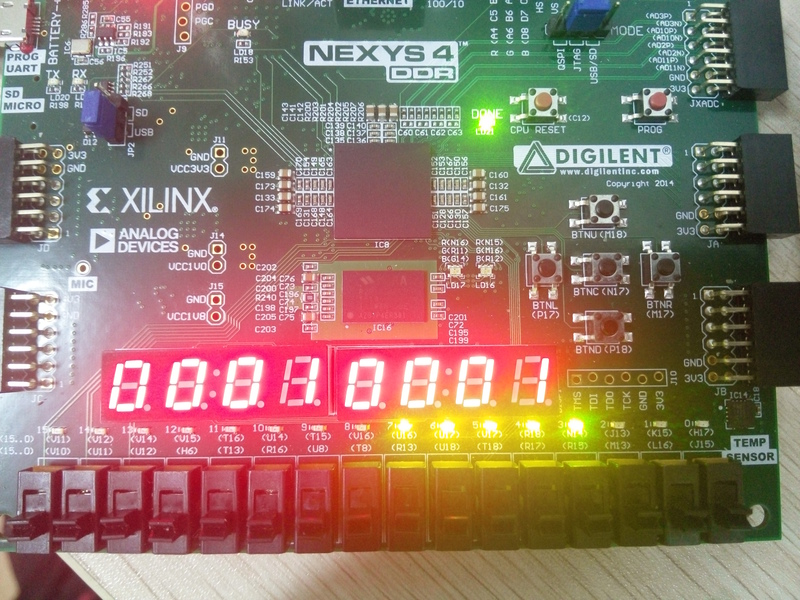
\includegraphics[width=5in]{figures/download/03.jpg}
  \caption{指令1在t4时}
  \label{fig:down:03}
\end{figure}

由图\ref{fig:down:03}可以看出,在t4时,PC\_update为'1',此时PC会被修改。

\section{指令2:JZ R0, 0x03(地址0x0001)}

\begin{figure}[H]
  \centering
  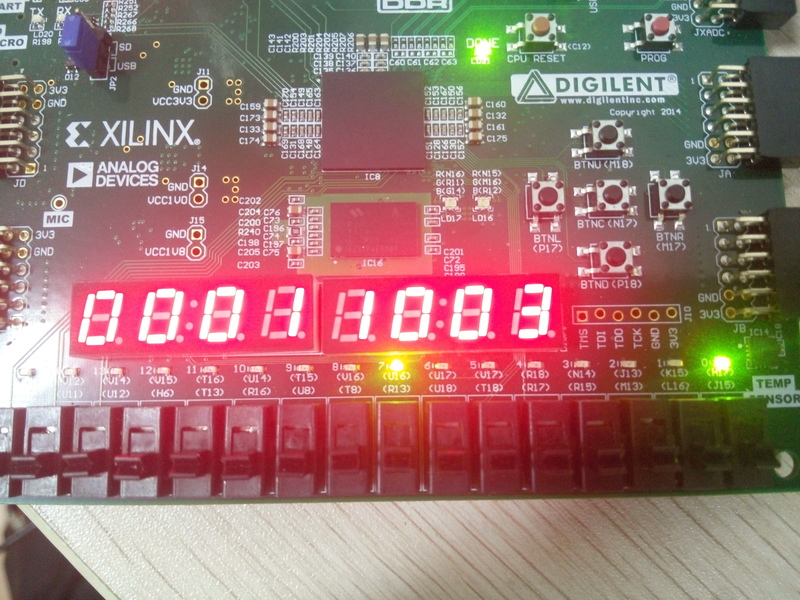
\includegraphics[width=5in]{figures/download/10.jpg}
  \caption{指令2在t1时}
  \label{fig:down:10}
\end{figure}

在执行这条指令时,由于R0初始化为0,故PC被修改0x0003。

\section{指令3:MVI R0, 0x01(地址0x0003)}

此时PC=0x0003,IR=0x4001。

\section{指令4:JZ R0, 0x02(地址0x0004)}

\begin{figure}[H]
  \centering
  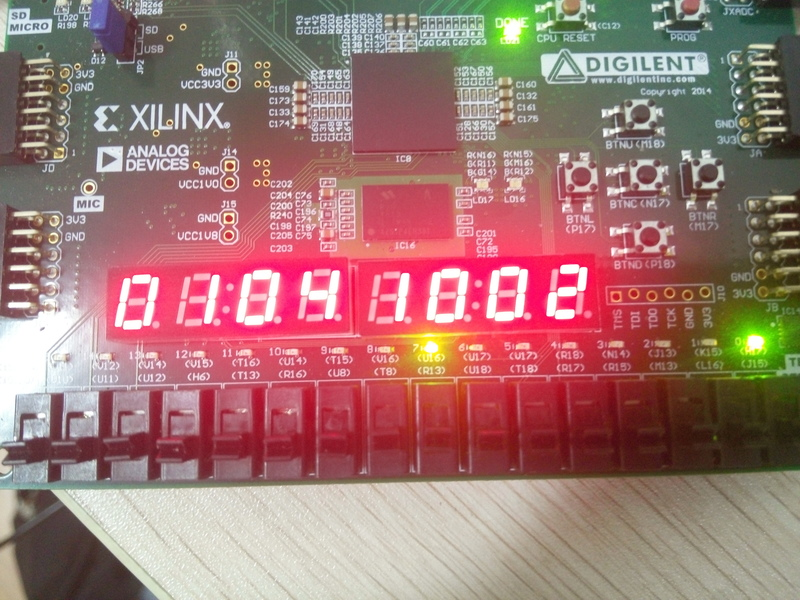
\includegraphics[width=5in]{figures/download/30.jpg}
  \caption{指令4在t1时}
  \label{fig:down:30}
\end{figure}

此时R0为1,故跳转条件不成立,PC在该指令结束后应为0x0005。

\section{指令5:MVI R7, 0x07(地址0x0005)}

\begin{figure}[H]
  \centering
  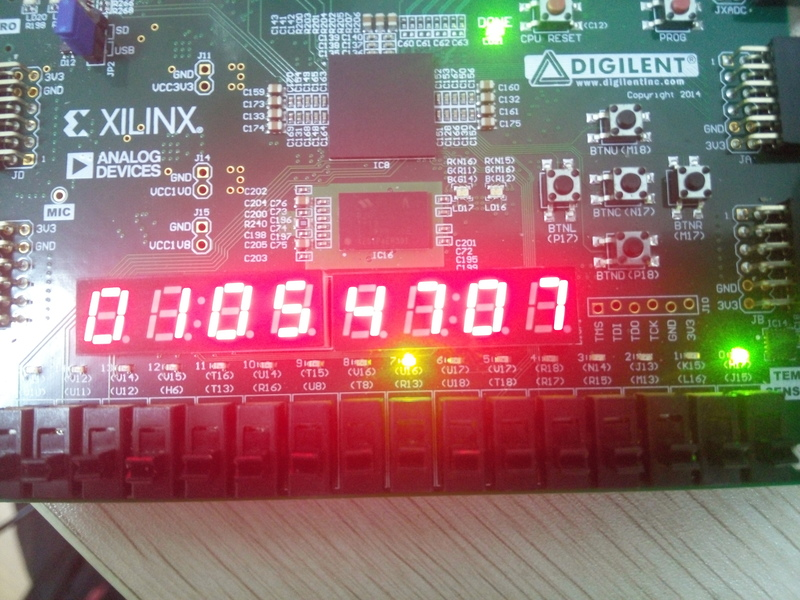
\includegraphics[width=5in]{figures/download/40.jpg}
  \caption{指令5在t1时}
  \label{fig:down:40}
\end{figure}

\begin{figure}[H]
  \centering
  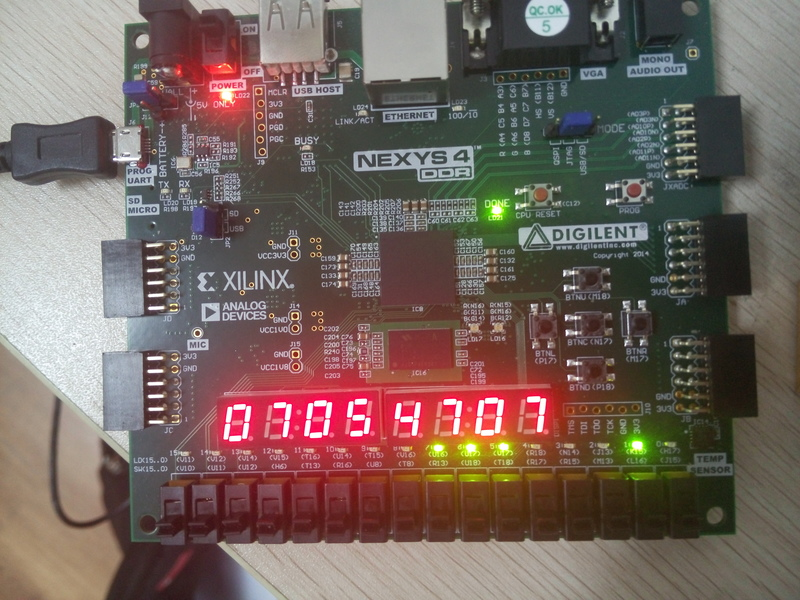
\includegraphics[width=5in]{figures/download/41.jpg}
  \caption{指令5在t2时}
  \label{fig:down:41}
\end{figure}

如图\ref{fig:down:41},在t2时,ALU\_out为7。

\section{指令6:ADD R0, R7(地址0x0006)}

\begin{figure}[H]
  \centering
  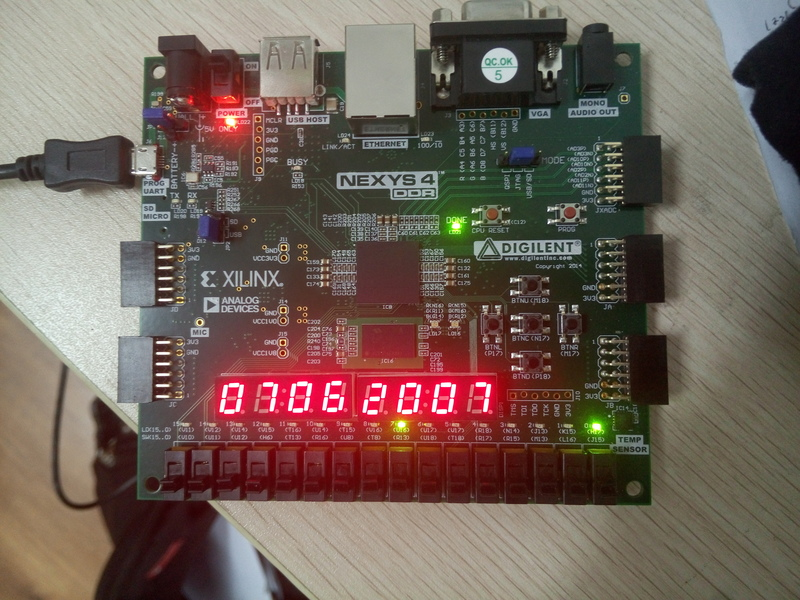
\includegraphics[width=5in]{figures/download/50.jpg}
  \caption{指令6在t1时}
  \label{fig:down:50}
\end{figure}

\begin{figure}[H]
  \centering
  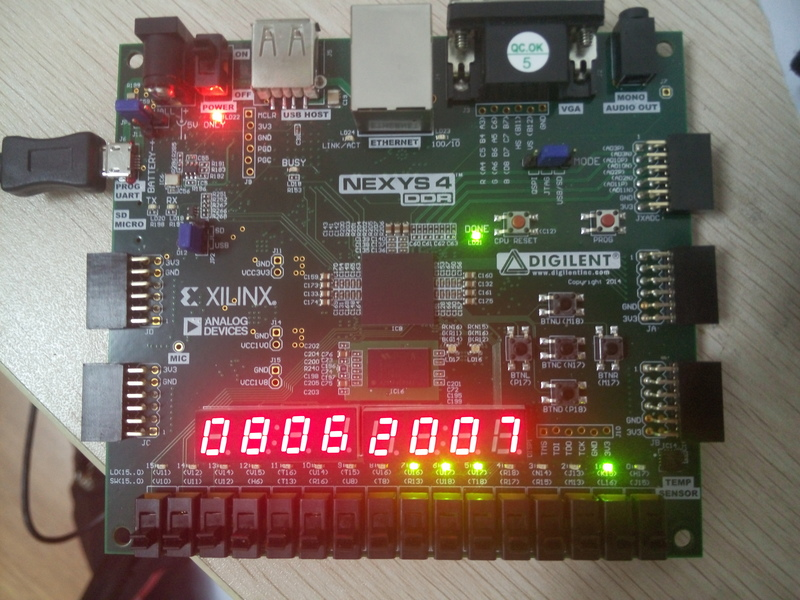
\includegraphics[width=5in]{figures/download/51.jpg}
  \caption{指令6在t2时}
  \label{fig:down:51}
\end{figure}

如图\ref{fig:down:51},在t2时,ALU\_out等于R0+R7=8。

\section{指令7:OUT R0, 0x1(地址0x007)}

\begin{figure}[H]
  \centering
  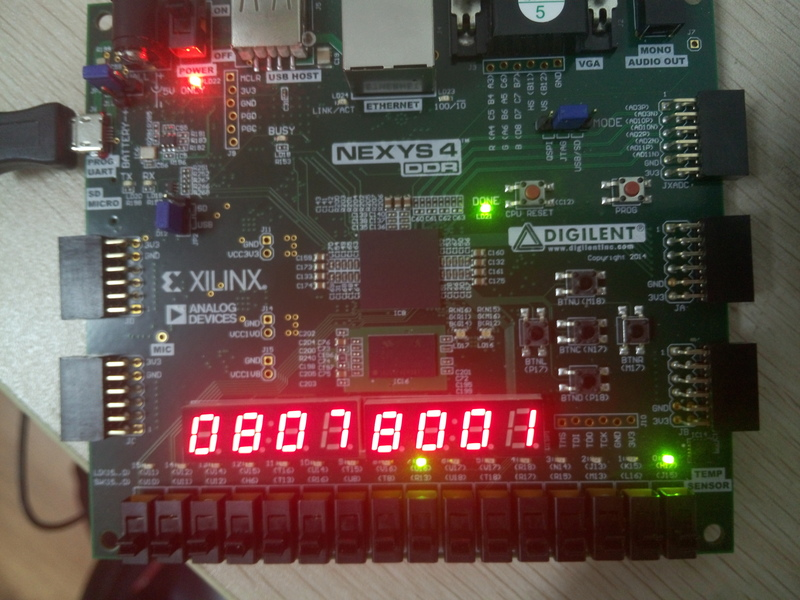
\includegraphics[width=5in]{figures/download/60.jpg}
  \caption{指令7在t1时}
  \label{fig:down:60}
\end{figure}

\begin{figure}[H]
  \centering
  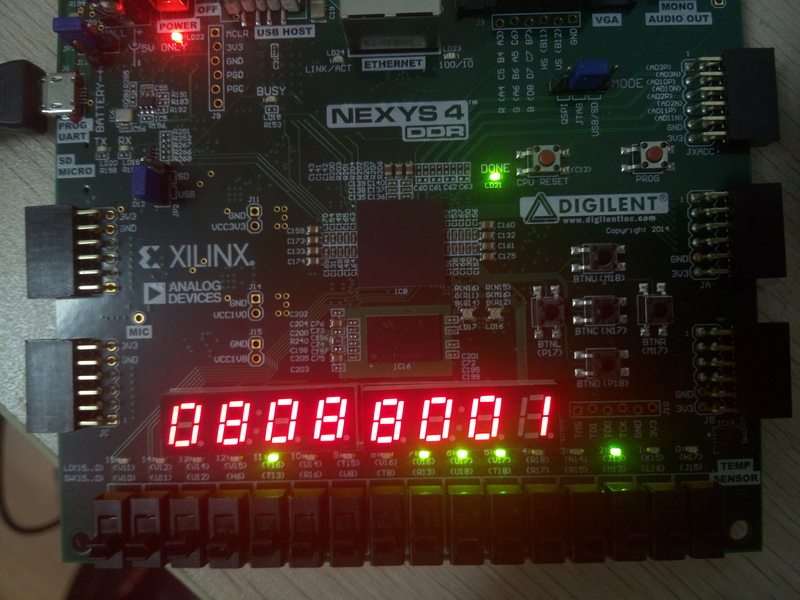
\includegraphics[width=5in]{figures/download/62.jpg}
  \caption{指令7在t2时}
  \label{fig:down:62}
\end{figure}

如图\ref{fig:down:62}所示,此时输出端口结果为0x08,恰为R0的值。

\section{指令8:STA R7, 0x0c(地址0x008)}

\begin{figure}[H]
  \centering
  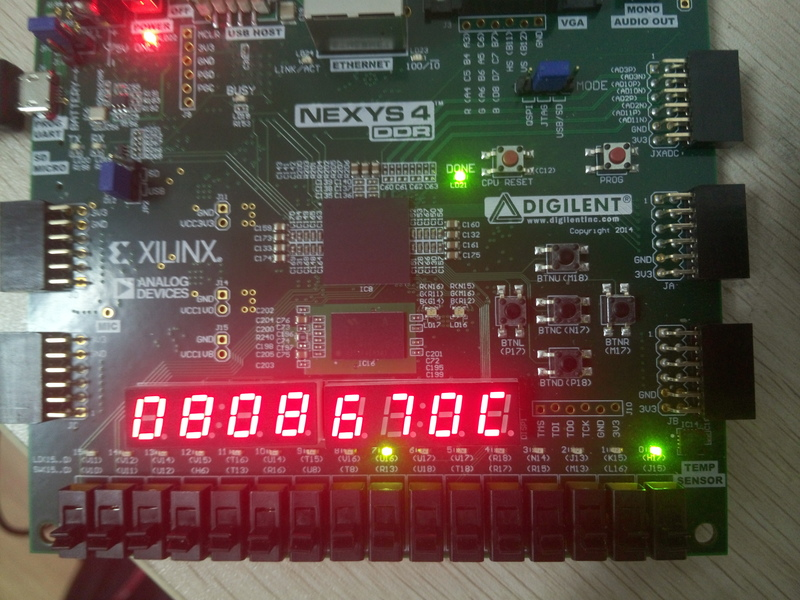
\includegraphics[width=5in]{figures/download/70.jpg}
  \caption{指令8在t1时}
  \label{fig:down:70}
\end{figure}

\begin{figure}[H]
  \centering
  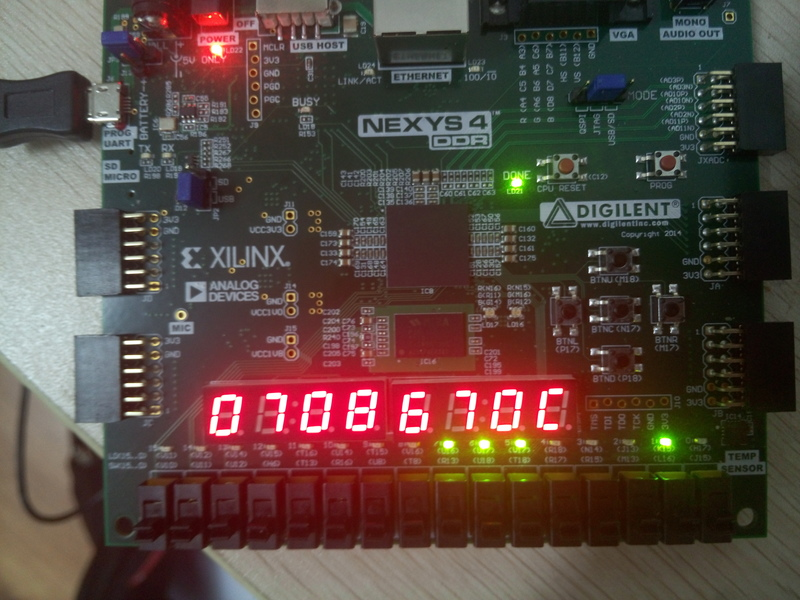
\includegraphics[width=5in]{figures/download/71.jpg}
  \caption{指令8在t2时}
  \label{fig:down:71}
\end{figure}

\begin{figure}[H]
  \centering
  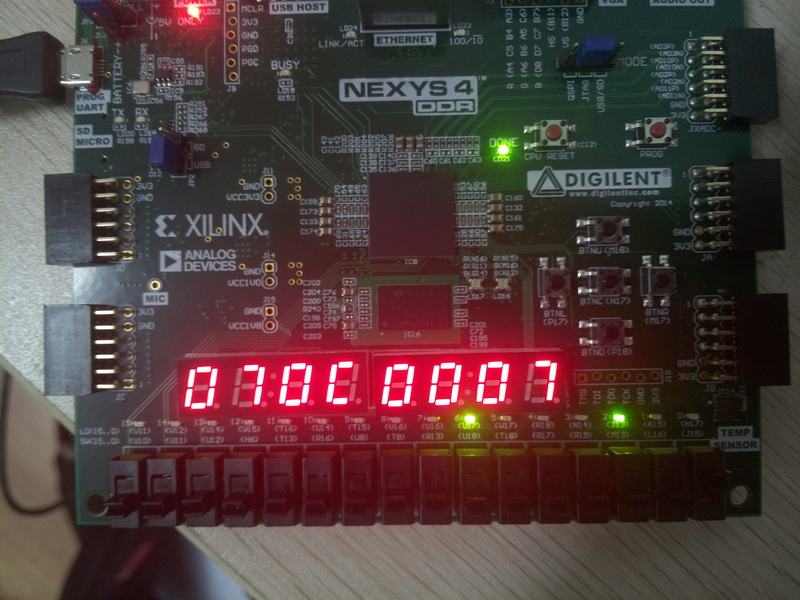
\includegraphics[width=5in]{figures/download/72.jpg}
  \caption{指令8在t3时}
  \label{fig:down:72}
\end{figure}

如图\ref{fig:down:72},此时地址总线为0x070c,数据总线为0x0007。

\section{指令9:LDA R1, 0x0c(地址0x009)}

\begin{figure}[H]
  \centering
  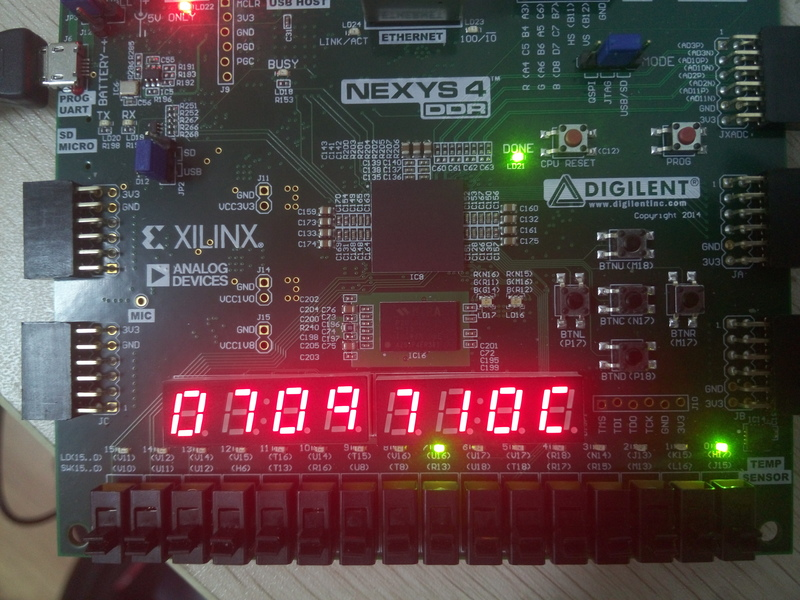
\includegraphics[width=5in]{figures/download/80.jpg}
  \caption{指令9在t1时}
  \label{fig:down:80}
\end{figure}

\section{指令10:SUB R1, R0(地址0x00a)}

\begin{figure}[H]
  \centering
  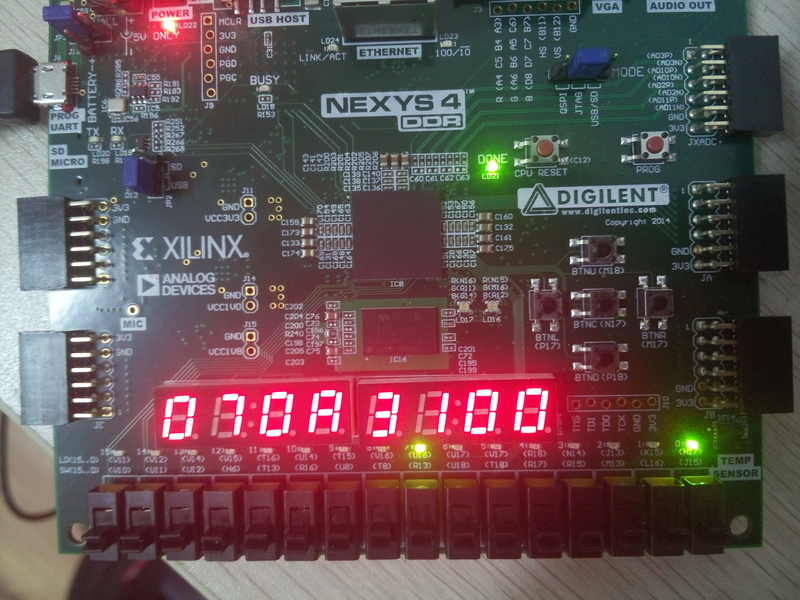
\includegraphics[width=5in]{figures/download/90.jpg}
  \caption{指令10在t1时}
  \label{fig:down:90}
\end{figure}

\section{指令11:OUT R1, 0x1(地址0x00b)}

\begin{figure}[H]
  \centering
  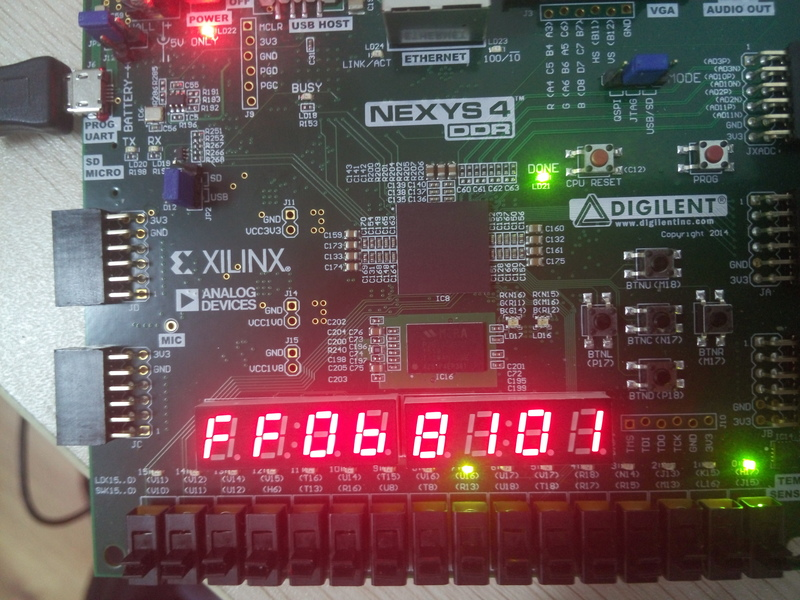
\includegraphics[width=5in]{figures/download/a0.jpg}
  \caption{指令11在t1时}
  \label{fig:down:a0}
\end{figure}

\begin{figure}[H]
  \centering
  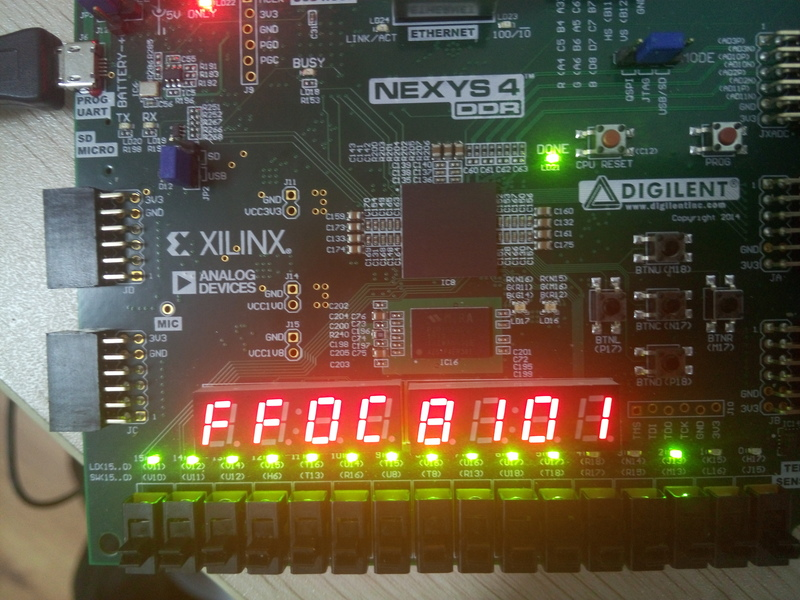
\includegraphics[width=5in]{figures/download/a2.jpg}
  \caption{指令11在t3时}
  \label{fig:down:a2}
\end{figure}


\section{指令12:IN R2, 0x1(地址0x00c)}

\begin{figure}[H]
  \centering
  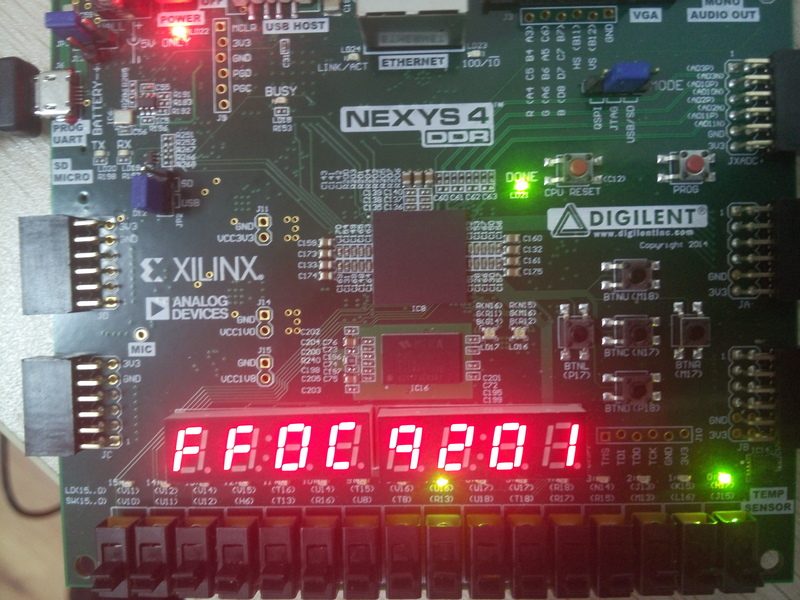
\includegraphics[width=5in]{figures/download/b0.jpg}
  \caption{指令12在t1时}
  \label{fig:down:b0}
\end{figure}

\begin{figure}[H]
  \centering
  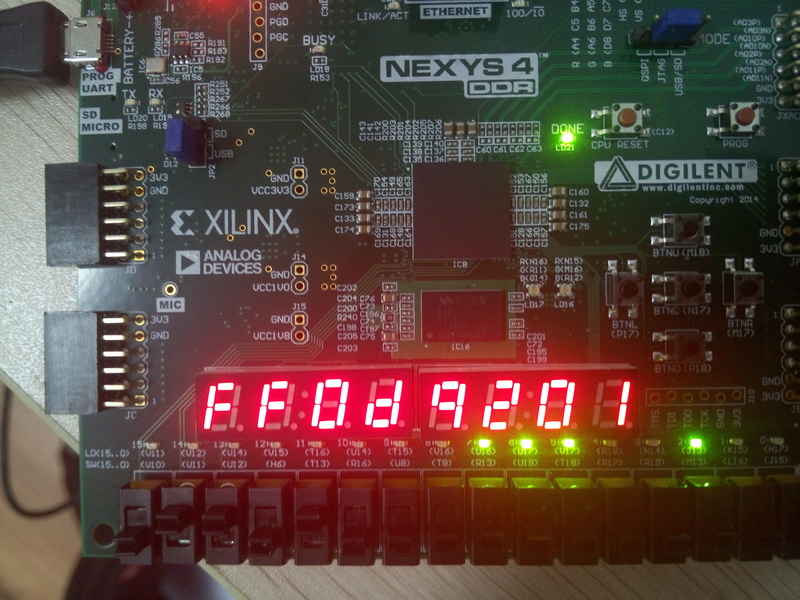
\includegraphics[width=5in]{figures/download/b2.jpg}
  \caption{指令12在t3时}
  \label{fig:down:b2}
\end{figure}


\section{指令13:OUT R2, 0x1(地址0x00d)}

\begin{figure}[H]
  \centering
  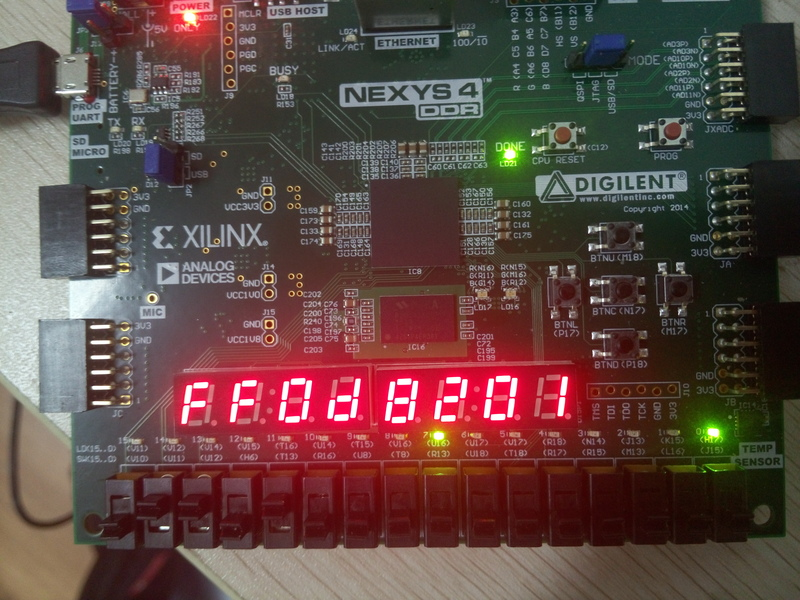
\includegraphics[width=5in]{figures/download/c0.jpg}
  \caption{指令13在t1时}
  \label{fig:down:c0}
\end{figure}

\begin{figure}[H]
  \centering
  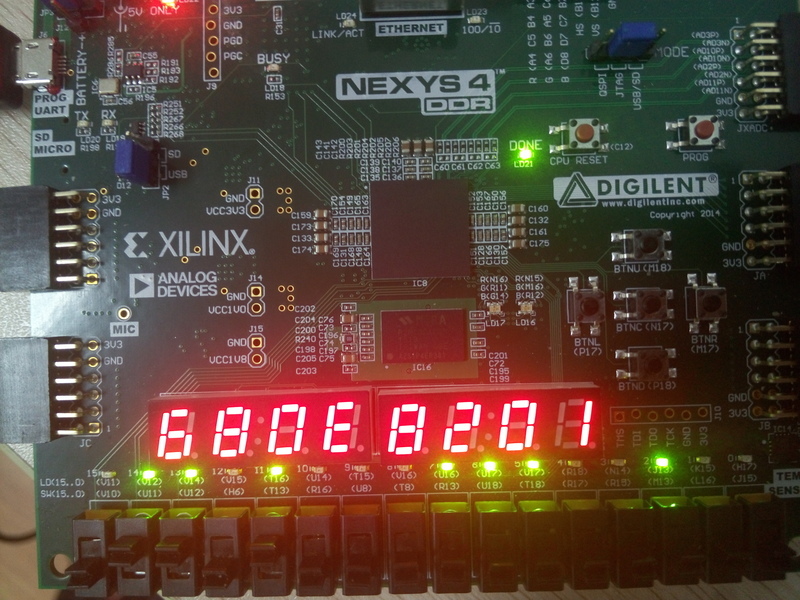
\includegraphics[width=5in]{figures/download/c2.jpg}
  \caption{指令13在t3时}
  \label{fig:down:c2}
\end{figure}

如图\ref{fig:down:c2},执行本指令时的IO输出恰为执行上一指令时的IO输入。

\chapter{实验中遇到的问题}

\section{关于PC何时自加}

由于一直担心在读IR时,内存的地址要给得十分稳定,怕在t2上升沿PC自加,会造成问题,纠结了很长时间。最后询问老师,老师告诉我可以在t3使用组合逻辑让PC自加,由此问题解决。虽然甚至还没开始写代码,但这种问题想不明白,总是不敢动手写,在这里要谢谢老师的耐心指导。

\section{关于when...else...语句}

一直以为在使用when...else...语句时,最后如果不加一个else,例如:

\begin{minted}{VHDL}
   Z <= A when X > 5;
\end{minted}

vhdl会默认加一个锁存器保存结果。然而,在下载时在这种语句上出了问题,于是我查阅资料,在这个网页\footnote{\url{http://www.ics.uci.edu/~jmoorkan/vhdlref/cond_s_a.html}}中看到,不写else是不对的。改正了之后(将某些OUT信号改成了buffer,when...else..语句后加了else)结果就正常了。

\section{产生200MHz的信号供DDR2内存使用}

由于DDR2内存需要一个频率为200MHz的时钟信号输入,而板子上只有一个频率为100MHz的时钟信号。查阅资料发现又一个IP核叫做clk\_wiz\_0,可以产生更高频率的时钟信号。然后顺带学了一下IP核的使用,最后问题解决。

\section{DDR2内存读写结果不正确}

开始用DDR2内存时,尝试过往里写入信息,然后再读,发现信息被修改了。百思不得其解,查阅文档也没找到想要的答案。最后闲着没事算了一下128MB的内存如果按字编址需要多少根地址线,才发现Nexys 4上的内存,虽然数据线宽度为16,但却是用字节编址的。所以访存地址*2,问题得以解决。

%%%=== 参考文献 ========%%%
\cleardoublepage\phantomsection
\addcontentsline{toc}{chapter}{参考文献}
\begin{thebibliography}{00}

\bibitem{web1} Xilinx Inc., \url{http://www.xilinx.com/support/documentation/ip_documentation/mig_7series/v2_1/ug586_7Series_MIS.pdf}
\bibitem{book1} 雷思磊. 自己动手写CPU[M]. 电子工业出版社, 2014.
\bibitem{book2} RandalE.Bryant, DavidO'Hallaron, 龚奕利,等. 深入理解计算机系统[J]. 2004.

\end{thebibliography}

% !Mode:: "TeX:UTF-8"
%%%%%%%%%%%%%%%%%%%%%%%%%%%%-------致谢--------%%%%%%%%%%%%%%%%%%%%%%%%%%%%%%%%

\acknowledgement
\addcontentsline{toc}{chapter}{致谢}

感谢罗丹彦老师和助教学长的耐心指导,实验5的完成离不开他们的指点。











 %%%致谢

\cleardoublepage
\end{document}
